%%%%%%%%%%%%%%%%%%%%%%%%%%%%%%%%%%%%%%%%%
% Short Sectioned Assignment LaTeX Template Version 1.0 (5/5/12)
% This template has been downloaded from: http://www.LaTeXTemplates.com
% Original author:  Frits Wenneker (http://www.howtotex.com)
% License: CC BY-NC-SA 3.0 (http://creativecommons.org/licenses/by-nc-sa/3.0/)
%%%%%%%%%%%%%%%%%%%%%%%%%%%%%%%%%%%%%%%%%

% \documentclass[paper=a4, fontsize=11pt]{scrartcl} % A4 paper and 11pt font size
\documentclass[11pt, a4paper]{book}
\usepackage[T1]{fontenc} % Use 8-bit encoding that has 256 glyphs
\usepackage[utf8]{inputenc}
\usepackage{fourier} % Use the Adobe Utopia font for the document - comment this line to return to the LaTeX default
\usepackage{listings} % para insertar código con formato similar al editor
\usepackage[spanish, es-tabla]{babel} % Selecciona el español para palabras introducidas automáticamente, p.ej. "septiembre" en la fecha y especifica que se use la palabra Tabla en vez de Cuadro
\usepackage{url} % ,href} %para incluir URLs e hipervínculos dentro del texto (aunque hay que instalar href)
\usepackage{graphics,graphicx, float} %para incluir imágenes y colocarlas
\usepackage[gen]{eurosym} %para incluir el símbolo del euro
\usepackage{cite} %para incluir citas del archivo <nombre>.bib
\usepackage{enumerate}
\usepackage{hyperref}
\usepackage{graphicx}
\usepackage{tabularx}
\usepackage{booktabs}
\usepackage{setspace}
\usepackage{ragged2e}
\usepackage{amsmath}
\usepackage[nottoc,notlot,notlof]{tocbibind}
\usepackage{nomencl}

% Definir el estilo para tener líneas de 80 caracteres
\newcommand{\lineasochenta}{\setstretch{1.2}\setlength{\parindent}{0pt}\RaggedRight\setlength{\emergencystretch}{1em}\setlength{\parskip}{1em}}


\usepackage[table,xcdraw]{xcolor}
\hypersetup{
	colorlinks=true,	% false: boxed links; true: colored links
	linkcolor=black,	% color of internal links
	urlcolor=cyan		% color of external links
}
\renewcommand{\familydefault}{\sfdefault}
\usepackage{fancyhdr} % Custom headers and footers
\pagestyle{fancyplain} % Makes all pages in the document conform to the custom headers and footers
\fancyhead[L]{} % Empty left header
\fancyhead[C]{} % Empty center header
\fancyhead[R]{Jose Antonio Jordan Fernández} % My name
\fancyfoot[L]{} % Empty left footer
\fancyfoot[C]{} % Empty center footer
\fancyfoot[R]{\thepage} % Page numbering for right footer
%\renewcommand{\headrulewidth}{0pt} % Remove header underlines
\renewcommand{\footrulewidth}{0pt} % Remove footer underlines
\setlength{\headheight}{13.6pt} % Customize the height of the header
%\setlength{\textwidth}{350pt} % Prueba con 400pt
%\setlength{\textwidth}{480pt} % Ancho de página de 80 caracteres a 6pt por carácter


\usepackage{titlesec, blindtext, color}
\definecolor{gray75}{gray}{0.75}
\newcommand{\hsp}{\hspace{20pt}}
\titleformat{\chapter}[hang]{\Huge\bfseries}{\thechapter\hsp\textcolor{gray75}{|}\hsp}{0pt}{\Huge\bfseries}
\setcounter{secnumdepth}{4}
\usepackage[Lenny]{fncychap}


\begin{document}

	% Plantilla portada UGR
	\begin{titlepage}
\newlength{\centeroffset}
\setlength{\centeroffset}{-0.5\oddsidemargin}
\addtolength{\centeroffset}{0.5\evensidemargin}
\thispagestyle{empty}

\noindent\hspace*{\centeroffset}\begin{minipage}{\textwidth}

\centering
\includegraphics[width=0.9\textwidth]{logos/logo_ugr.jpg}\\[1.4cm]

\textsc{ \Large TRABAJO FIN DE GRADO\\[0.2cm]}
\textsc{ GRADO EN INGENIERIA INFORMATICA}\\[1cm]

{\Huge\bfseries Claqueta \\}
\noindent\rule[-1ex]{\textwidth}{3pt}\\[3.5ex]
{\large\bfseries Sistema de reseñas de
audiovisual con sistema de
recomendación }
\end{minipage}

\vspace{2.5cm}
\noindent\hspace*{\centeroffset}
\begin{minipage}{\textwidth}
\centering

\textbf{Autor}\\ {José Antonio Jordan Fernández}\\[2.5ex]
\textbf{Director}\\ {Juan Julián Merelo Guervós}\\[2cm]
\includegraphics[width=0.3\textwidth]{logos/etsiit_logo.png}\\[0.1cm]
\textsc{Escuela Técnica Superior de Ingenierías Informática y de Telecomunicación}\\
\textsc{---}\\
Granada, junio de 2024
\end{minipage}
\end{titlepage}


	% Plantilla prefacio UGR
	\cleardoublepage


\begin{titlepage}

\setlength{\centeroffset}{-0.5\oddsidemargin}
\addtolength{\centeroffset}{0.5\evensidemargin}
\thispagestyle{empty}

\noindent\hspace*{\centeroffset}\begin{minipage}{\textwidth}

\centering

\includegraphics[width=0.3\textwidth]{logos/claqueta_logo.png}\\[1.cm]

\textsc{ \Large TRABAJO FIN DE GRADO\\[0.2cm]}
\textsc{ GRADO EN INGENIERIA INFORMATICA}\\[1cm]

{\Huge\bfseries Claqueta \\}
\noindent\rule[-1ex]{\textwidth}{3pt}\\[3.5ex]
{\large\bfseries Sistema de reseñas de
audiovisual con sistema de
recomendación }
\end{minipage}

\vspace{2.5cm}
\noindent\hspace*{\centeroffset}
\begin{minipage}{\textwidth}
\centering

\textbf{Autor}\\ {José Antonio Jordan Fernández}\\[2.5ex]
\textbf{Director}\\ {Juan Julián Merelo Guervós}\\[2cm]
\includegraphics[width=0.3\textwidth]{logos/etsiit_logo.png}\\[0.1cm]
\textsc{Escuela Técnica Superior de Ingenierías Informática y de Telecomunicación}\\
\textsc{---}\\
Granada, junio de 2024
\end{minipage}
\end{titlepage}


\cleardoublepage

\thispagestyle{empty}


\begin{center}
{\large\bfseries Claqueta \\ Sistema de reseñas de
audiovisual con sistema de
recomendación }\\
\end{center}
\begin{center}
Jose Antonio Jordan Fernández\\
\end{center}

%\vspace{0.7cm}

\vspace{0.5cm}
\noindent\textbf{Palabras clave}: \textit{cine, reseñas, recomendaciones, fiabilidad, entretenimiento, software libre, historias de usuario, historias de desarrollador, agile, PMV}
\vspace{0.7cm}

\noindent\textbf{Resumen}\\

Claqueta es una plataforma creada bajo un marco de desarrollo específico para resolver ciertas necesidades de distintos usuarios, basada en el consumo de contenido cinematográfico, busca recomendar contenido bajo sus preferencias a los distintos usuarios activos. Fomentar la libre opinión sobre el contenido a través de reseñas, y lograr formar una comunidad unida por el cine. Para ello se da una pequeña introducción donde se plantea de forma superficial el problema que se desea resolver, los objetivos a cumplir con la solución a dicho problema, y bajo que marco de desarrollo se realizara dicha solución. Se describe en más detalle el problema, las personas que se ven afectadas por él y sus historias o necesidades, también se echa un vistazo al mercado y como intentan otras plataformas resolver dicho problema. Se orienta la planificación del proyecto y se lleva a cabo finalmente su implementación, tras la que se echa una mirada al inicio del proyecto para comprobar los resultados obtenidos y aportaciones futuras.
	

\cleardoublepage

\begin{center}
	{\large\bfseries Claqueta\\Audiovisual review system with recommendation system}\\
\end{center}
\begin{center}
	José Antonio Jordan Fernández\\
\end{center}
\vspace{0.5cm}
\noindent\textbf{Keywords}: \textit{cinema, reviews, recommendations, reliability, entertainment, free software,user stories, developer stories, agile, PMV}
\vspace{0.7cm}

\noindent\textbf{Abstract}\\

Claqueta is a platform created under a specific development framework to solve certain needs of different users, based on the consumption of film content, seeks to recommend content based on their preferences to different active users. Encourage free opinion on the content through reviews, and achieve to form a community united by the cinema. For this purpose, a short introduction is given where the problem to be solved is superficially stated, the objectives to be met with the solution to the problem, and the development framework under which the solution will be carried out. It describes in more detail the issue, the people who are affected by it and their stories or needs, and also takes a look at the market and how other platforms are trying to solve the problem. The project planning is guided, and finally the implementation is carried out, after which a look back to the beginning of the project to check the results achieved and future contributions.

\cleardoublepage


\thispagestyle{empty}

\noindent\rule[-1ex]{\textwidth}{2pt}\\[4.5ex]

Yo,\textbf{José Antonio Jordan Fernández}, alumno de la titulación en Ingeniería Informática de la Escuela Técnica 
Superior de Ingenierías Informática y de Telecomunicación de la Universidad de Granada, con DNI
20886138E, autorizo la ubicación de la siguiente copia de mi Trabajo
Fin de Grado en la biblioteca del centro para que pueda ser consultada por
las personas que lo deseen. 



\vspace{5cm}

\noindent \textbf{Fdo: José Antonio Jordan Fernández }

\vspace{1cm}

 \begin{center}
     \noindent Granada a 24 de junio de 2024
 \end{center}

\cleardoublepage

\thispagestyle{empty}

\noindent\rule[-1ex]{\textwidth}{2pt}\\[4.5ex]

D. \textbf{Juan Julián Merelo Guervós}, Profesor del departamento de Ingeniería de Computadores, Automática y Robótica 

\vspace{0.5cm}

\textbf{Informo:}

\vspace{0.5cm}

Que el presente trabajo, titulado \textit{\textbf{Claqueta, Sistema de reseñas de audiovisual con sistema de 
recomendación}}, ha sido realizado bajo mi supervisión por \textbf{José Antonio Jordan Fernández}, y autorizo la defensa 
de dicho trabajo ante el tribunal
que corresponda.

\vspace{0.5cm}

Y para que conste, expiden y firman el presente informe en Granada a Junio de 2024.

\vspace{1cm}

\textbf{El director: }

\vspace{5cm}

\noindent \textbf{(Juan Julián Merelo Guervós)}

\chapter*{Agradecimientos}

Quiero agradecer este trabajo a mi familia que siempre ha estado cuando la he necesitado, a mi pareja que siempre creyó 
en mí, incluso cuando ni yo mismo lo hacía.
También se lo agradezco a mi tutor JJ por soportarme día sí y día también, y enseñarme realmente como debe realizarse un proyecto de software y que lo importante no es cantidad, sino calidad.

Por último, gracias a la UGR y en especial a la ETSIIT por otorgarme el conocimiento y las habilidades para terminar esta etapa y lanzarme al mundo laboral.




	% Índice de contenidos
	\newpage
	\tableofcontents

	% Índice de imágenes y ecuaciones
	\newpage
	\listoffigures
 
	% Si hay suficientes se incluirá dicho índice
    
    \listoftables
	 
	\newpage
    \makenomenclature
    \renewcommand{\nomname}{Índice de Operaciones}
    \newcommand{\eqindex}[1]{\nomenclature{#1}{\pageref{#1}}}
    \printnomenclature[2cm]
    \newpage

	% Introducción 
	

\chapter{Introducción}

Gran parte del entretenimiento se deriva del propio contenido audiovisual, ya sean series, películas,
documentales, recitales, conciertos, etc. Un grupo de personas simplemente se conforma con visualizar el 
contenido, pero existe otro grupo que no satisface su necesidad de entretenimiento solo visionando estos 
productos. Por ello necesitan algo más, ese algo es compartir su experiencia, su opinión acerca del 
producto consumido, con sus allegados y amigos. Pero como es posible que lo hagan con otros usuarios que 
sientan la misma necesidad de debatir o especular sobre la obra audiovisual que han visto.

A través de reseñas. \textit{''Una reseña cinematográfica es una reacción instantánea de un espectador a 
una película. Es como el chisme en una cena, cuando te vuelves hacia la persona de al lado y le 
preguntas '¿qué pensaste?' Una reseña de cine es una respuesta a una experiencia compartida de la 
película, no es una síntesis de los elementos que la componen''}. Definición de reseña por 
\textit{''Roger Ebert''} un reconocido escritor, y critico de cine de Estados Unidos \cite{REwebsite}. 

Esa necesidad de comentar la obra que acababas de visualizar, comenzó a finales del siglo XIX y a 
principios del siglo XX, ya que se popularizó el cine como forma de entretenimiento. Creando así la 
necesidad de comentar, analizar y discutir estas películas. Gracias a la concepción del cine como un 
arte y no solo como un entretenimiento a principio de los años 20 por los críticos franceses, entre los 
que se encontraba \textit{''Louis Delluc''}, periodista, director y critico francés \cite{LouisD}. 
Surgieron entre los años 20 y 30 críticos en otros países como Reino Unido y Estados Unidos como el 
ganador del premio Pulitzer en 1958 por su novela autobiográfica \textit{''James Agee''} \cite{JamesA}. 

En el titulado \begin{otherlanguage}{english}``\textit{A VERY SHORT HISTORY OF FILM 
CRITICISM}''\end{otherlanguage}\cite{3BrothersArticle}\footnote{\url{https://3brothersfilm.com/blog/2018/7/23/7rnnqs20722u62gz2hhwmrmwar1ut4}}. 
Encontramos como el autor nos cuenta como ha evolucionado la crítica cinematográfica desde la época del 
famoso crítico \textit{''Roger Ebert''} hasta la era de las redes sociales. El autor trata de explicar 
que la crítica cinematográfica ha seguido siendo importante y evoluciona a lo largo de los años. Nos 
remarca que la crítica cinematográfica era más elitista y se enfocaba en películas de arte y ensayo, un 
tipo de cine que no ofrece una narración dramática ni una representación histórica del mundo, sino una 
reflexión sobre el propio medio. Diferenciándose de la narrativa clásica en varios puntos, siendo 
narrativa de arte y ensayo frente a narrativa clásica. Casualidad frente a  causalidad, un final 
abierto frente a un final cerrado, tiempo no lineal frente a tiempo literal, conflicto interno frente a 
conflicto externo, un protagonista pasivo frente a un protagonista activo, una realidad ambigua frente 
a una realidad coherente y el centro de la historia es el personaje y no la acción mientras que por la 
narrativa clásica se centra en la acción y no en el personaje. Con el tiempo la crítica se extendió y 
se añadieron a su abanico las películas comerciales. La influencia de \textit{''Roger Ebert''} ayudo a 
popularizar la crítica cinematográfica en Estados Unidos gracias a sus escritos y a sus programas de 
televisión. 

A lo largo del tiempo, estos críticos han realizado un gran trabajo en la industria cinematográfica, ya 
que no solo han servido de guía para los espectadores, llevándolos hacia las películas más destacadas, 
gracias a su perspectiva crítica sobre estas. Si no que también has desempeñado un papel importante en 
el desarrollo de la teoría del cine y la crítica literaria. Influyendo así en la forma en que se piensa 
y se habla sobre el cine en la cultura general. Se podría decir que el desarrollo del cine fue el que 
permitió que apareciera el mundo de las críticas cinematográficas, siendo una parte importante de la 
industria e importante para construir nuestra parte crítica dirigida a estas obras cinematográficas. Las 
herramientas que se usan para realizar estas reseñas también se han desarrollado a lo largo del tiempo, 
desde las herramientas más básicas de escritura, papel y pluma, pasando por la máquina de escribir, uso 
de grabadoras y cámaras, la llegada del ordenador de sobremesa y llegando hasta el ordenador portátil. 
Estas herramientas han permitido que las opiniones de los críticos lleguen cada vez a más gente en el 
menos tiempo posible. El mayor salto fue la aparición de internet, de manera que podían compartir su 
opinión llegando a casi todas las partes del mundo, incluso gracias a nuevas tecnologías que han ido 
apareciendo como el \begin{otherlanguage}{english}``\textit{streamming}''\end{otherlanguage} o las redes 
sociales comentadas en el artículo mencionado con anterioridad, que ofrecen realizar criticas en tiempo 
real, siendo una herramienta con mucho potencial y al alcance de la mano de cualquier usuario.

De este modo existen varios espacios famosos como IMDb\cite{IMDbWeb}, web por excelencia conocida por 
ser una de las pioneras en internet. Contiene una gran cantidad de información sobre todo lo relacionado 
con el cine y las series. Una masiva información de calidad al alcance de cualquier usuario, desde si 
buscas a un actor en particular, cierto director o simplemente quieres comentar lo mucho que te ha 
entusiasmado una película que acabas de ver. También posee un sistema de ranking mediante el cual los 
usuarios pueden puntuar cada reseña, estableciendo así cierta reputación a usuarios que tengan una 
puntuación decente gracias a sus opiniones fundadas sobre la obra cinematográfica. Otros espacios 
similares serían Rotten Tomatoes\cite{RottenTWeb} o una web española como SensaCine\cite{SSweb} en las 
que podemos realizar todas las actividades mencionadas antes.

Como se mencionó antes, la llegada de internet y las redes sociales ha permitido que la crítica 
cinematográfica sea más accesible y democrática. Pero también ha traído una ingente cantidad de 
información, provocando una sobrecarga de información y una perdida de profundidad crítica, debido a la 
fugacidad y la celeridad de las redes sociales, han conducido a la crítica cinematográfica a que sea 
más superficial y menos reflexiva. Aun así, la crítica cinematográfica sigue siendo importante en la 
época de las redes sociales, ya que puede ayudar a sus consumidores a comprender mejor el mundo en el 
que viven, descubrir películas y directores interesantes. Por lo que el artículo mencionado 
anteriormente concluye afirmando que la critica, a pesar de haber cambiado a lo largo de los años, 
continúa siendo una forma valiosa de arte y análisis cultural, y anima a sus lectores a buscar y 
compartir reseñas sobre obras cinematográficas que visualicen.

Por ello se plantea un problema, los usuarios necesitan complacer su necesidad de compartir su opinión 
sobre toda obra cinematográfica que ven, sin impedimentos en cualquier lugar y en cualquier momento. 
Existen otros usuarios cuyas necesidades se encuentran en discernir si ven o no una película, esta 
decisión recae sobre esas opiniones de otros usuarios que ya han visto el contenido. Así, el usuario 
que necesita una recomendación para finalmente visualizar o no algún contenido audiovisual recurren a 
estas críticas, ya les agraden o no les ayudan a tomar una decisión. Por lo que la reseña influye mucho 
en la deliberación de los usuarios dubitativos de ver cierto contenido.

\section{Motivación}

Desde muy pequeño siempre me ha gustado ver las cintas VHS que había en mi casa, desde que me las ponía 
mi familia, hasta que yo pude poner una y otra vez esas cintas, llegando a repetir la misma película 
infinidad de veces sin cansancio alguno. De alguna manera el cine es un mundo aparte en el que no hay 
nada más que la película que estás viendo en ese momento, no hay polémicas, problemas, agobios, estrés. 
Te desinhibes al completo y disfrutas de la película con los que te rodean, riendo, llorando, cantando 
o sintiendo, por esos personajes que hacemos nuestros cuando vemos alguna obra cinematográfica. 

Y de alguna manera el poder expresar lo que te ha parecido la obra que has visto y compartirlo con 
aquellas personas que se crucen con tu reseña y tengan la posibilidad de interactuar contigo y discutir 
sobre lo que ambos habéis visto. Me hace volver a esos tiempos en los que estás con amigos o familia 
comentando tranquilamente en casa, una película en la televisión. Al final solo estás viendo ficción, 
comedia, tristeza, alegría, terror, vidas, muertes. Siendo el objetivo de la obra, transmitir ese 
sentimiento y hacer que te evadas de lo demás. También es una herramienta muy fuerte en países con 
algún régimen opresor, siendo una manera de expresión, liberación, comunicación y protesta frente al 
gobierno que los oprime. Otro motivo es la integración cultural, existen idiomas o culturas que se 
pierden a lo largo del tiempo, si es posible resguardar dicho lenguaje y costumbres de aquellas 
culturas, aunque sea ficción, merecerá la pena para que persista en el tiempo y pueda ser visto por 
otros que no vivieron en esos tiempos. Recordando así tanto lo malo como lo bueno de la historia, 
pudiendo aprender de ello.

Y las reseñas sobre esas obras tendrían el poder de transmitir al resto del mundo el sentimiento 
producido por ese cine y conseguir que el público contribuya a la causa, presionando a la parte 
opresora o simplemente divulgando para que más gente disfrute de esas obras audiovisuales. Por tanto, 
el poder de la escritura, de la reseña en este caso, no es una minucia.


Cita de \textit{''Neil Gaiman''}\cite{NeilG} famoso escritor británico de ficción, novelas gráficas,
películas, teatro de audio...
\begin{verbatim}
    ``Solo escribiendo puedo hacer 
    que el mundo sea lo que debería ser''.
\end{verbatim}

De esta manera, toda persona que disfrute con el cine tendrá la oportunidad de compartir su experiencia 
tras la visualización de cualquier contenido, e instigar a otras personas a ver la obra o incluso a 
comentar lo que le ha parecido. Por ello, gracias a la época tecnológica en la que vivimos, es posible 
encontrar una solución a esa necesidad de cualquier usuario de manifestar su postura frente a las obras 
audiovisuales que consuma. Por lo que el motivo de este TFG es proporcionar una solución informática 
frente a esta necesidad de los usuarios, que sea útil, de manera que anime al usuario a usarla en su 
día a día para satisfacer su necesidad de compartir su experiencia y comentarlo con el resto de 
usuarios, sencilla y accesible para que todo usuario pueda utilizarla y acceder a ella de la forma más 
simple posible. Más debe ser una solución rentable y sostenible a largo plazo, y dispuesta a cambios 
suscitados por los usuarios que consumen dicha solución, para hacerla cada vez más robusta y apegada a 
las necesidades constantes de los usuarios. Pudiendo así ampliar la funcionalidad de la solución una 
vez resueltas las necesidades básicas. 

Este trabajo está dividido en tres partes diferenciadas:
\begin{itemize}
    \item En los \textbf{capítulos del 1 al 3} se debe comprender el trabajo y el contexto, describiendo 
    posteriormente el problema que se quiere resolver y los objetivos que se desean lograr. Tras esto, 
    en el estado del arte se analizarán las alternativas existentes en el mercado actualmente en 
    relación con espacios que permitan realizar críticas cinematográficas y compartirlas con los demás 
    usuarios, entendiendo de una mejor manera el dominio del problema.
    \item La segunda parte, construido por los \textbf{capítulos 4 y 5}, se concentran los matices 
    necesarios para llevar a cabo el proyecto, planificando el desarrollo, explicando la metodología a 
    usar, las distintas herramientas que se usaran en el proyecto y preparar el terreno para llevar a 
    cabo la implementación de la solución estudiada.
    \item Para terminar, en los \textbf{capítulos 6 y 7} se realizará todo el trabajo de desarrollo y se 
    evaluará la resolución de la propuesta, valorando si ha cumplido con las competencias y objetivos 
    propuestos.
\end{itemize}

Este proyecto es software libre, y está liberado con la licencia \cite{gplv3}. Y se puede encontrar en 
GitHub en este repositorio público \footnote{\url{https://github.com/JoseJordanF/Claqueta}}

	% Descripción del problema y hasta donde se llega
	\chapter{Descripción del problema}

En este capítulo se va a profundizar más en el problema que se plateaba en el primer capítulo y se 
expondrán los objetivos que se pretenden lograr en este proyecto

\section{Problema a resolver}

En la actualidad muchos usuarios disfrutan de visualizar cine y series, en casa, en el cine o en 
dispositivos móviles. Sin embargo, se suelen enfrentar al problema de decidir que ver y que no, ya que 
hay una ingente cantidad de opciones a su disposición. Aunque existen varias plataformas de reseñas 
cinematográficas, como mencionamos en el capítulo 1, muchas de ellas tienen una cantidad abrumadora de 
reseñas y es complicado determinar cuál es la opción dominante.

Además, algunas de estas plataformas pueden estar sesgadas o influenciadas por factores como la 
publicidad, los intereses corporativos y los prejuicios personales. Como resultado, los usuarios pueden 
no estar obteniendo una visión completa y objetiva de una obra cinematográfica o una serie antes de 
decidir verla.

Por lo que se necesita una aplicación, un espacio de reseñas cinematográficas que ofrezca a los 
usuarios una perspectiva completa y equilibrada de las películas y series que desean ver. Una 
aplicación que brinde tanto reseñas de usuarios como de críticos de cine profesionales, así como 
calificaciones y datos sobre dicha película o serie. Esto sería muy útil para ayudar a los usuarios a 
tomar decisiones informadas sobre que visualizar.

Resolviendo la base del problema, que los usuarios expresen sus opiniones no es más que el principio, 
ya que esta necesidad viene acompañada de aspectos más personalizables. Lo cual incide en más problemas 
de personalización de dicho espacio, como la facilidad de filtrar las reseñas, según las preferencias 
del usuario, siendo más eficaz en la ayuda de elección de películas y series. Obtener recomendaciones 
por parte de la aplicación, relacionadas con el contenido que consumes. Y que finalmente este espacio 
logre satisfacer toda necesidad del usuario, disfrutando así del espacio y llegando a promocionar su 
uso a usuarios cercanos a él.

Es muy importante escuchar al cliente, ya que son ellos los que van a explotar el producto, esto se 
verá más profundamente en el capítulo sobre la planificación, donde se hablara de la metodología usada.

Para una buena descripción del problema es esencial describir a las personas afectadas por dicho 
problema. Ya que ellos son los perjudicados, habrá que saber los dispositivos que usan, la 
accesibilidad que tienen a ellos. También las capacidades de estos usuarios y sus habilidades para 
poder definir el ámbito del problema y el propio problema.

Las personas afectadas por este problema que se les plantea cada vez que deciden consumir cualquier
contenido, ya sea para tomar decisiones o compartir su experiencia, serían aquellas a las que les 
gusta, les entretiene o les apasiona el cine u otra obra audiovisual. Y por supuesto le encanta 
compartir su experiencia con quien sea. También formarían parte del problema aquellas personas que 
necesitan de alguna recomendación para consumir cualquier producto audiovisual. Ellos necesitan una 
crítica contundente y objetiva del contenido para llegar a decidir si ver esa obra o no. También a 
estos grupos se unirían aquellos usuarios que les gusta discutir sobre la opinión de los demás acerca 
del contenido audiovisual. Existirán usuarios que pertenezcan a más de uno de estos grupos.

Actualmente, vivimos en una sociedad apegada a las redes sociales, las cuales han permitido la 
comunicación entre usuarios que en su vida jamás habrían podido encontrarse. En sí, el intercambio de 
ideas y el diálogo han sido expandidos a niveles mundiales, prácticamente no existe ninguna barrera
que no te permita comunicarte con quien quieras. La gran mayoría de personas afectadas por el problema 
tienen a su alcance un dispositivo móvil y la inmensa mayoría de usuarios usan como sistema operativo 
móvil ``\textit{Android}'' \cite{AndrvsIOS}. En este grupo encontraremos usuarios con una capacidad 
cognitiva más desarrollada que otros, ya sea por aprendizaje, experiencia o genética. Pero en general 
estos usuarios poseerán ciertas habilidades críticas y analíticas, habilidades argumentativas, 
comunicativas y expresivas. Habilidades ciertamente necesarias para las actividades que realiza este 
grupo de usuarios. Siendo todas estas habilidades fácilmente demostrables a través de  una red social. 
La edad de los usuarios puede variar bastante, ya que se encuentran en un rango muy amplio de edad. El 
mundo de la crítica y las recomendaciones respecto al cine u otros contenidos audiovisuales, como las 
series, es algo que le puede fascinar a usuarios de diversas edades, siempre cuando tenga una mínima 
edad para haber desarrollado algunas de las habilidades o capacidades mencionadas anteriormente. En
este rango, la gran mayoría se defenderán en la utilización de un dispositivo móvil, mientras que una 
pequeña parte puede tener problemas con el uso del teléfono móvil.

Gracias a ser una aplicación, los usuarios podrán usar la solución en cualquier lugar, siempre y 
cuando dispongan de conexión a Internet. Su uso generalmente no sería diario, se incrementaría cuando 
el usuario se disponga a ir al cine o ver una serie, siendo su forma de decidir si ver o no ese 
contenido. Tras visualizar el contenido audiovisual, también usaría la aplicación, ya que al usuario le 
gusta expresar su opinión sobre la película o serie que acaba de visualizar. Luego podríamos centrar su 
uso tanto a la previa visualización del contenido como tras su visualización. También podríamos añadir 
un punto de uso durante la visualización de la película o la serie, ya que la solución brinda datos 
relevantes sobre la obra, por lo que el usuario los podría consultar en cualquier momento. La 
aplicación también enviará notificaciones por las interacciones que tengan el resto de usuarios con tus 
reseñas, los usuarios que comentan tus reseñas o los usuarios que indican que les ha gustado o ha sido 
necesaria y relevante para la toma de decisiones de ese usuario. Hablando de las opciones 
personalizables sería una opción avisar de los estrenos de cine o series a través de notificaciones, 
siendo estas adaptables por el usuario.


\section{Historias de usuarios}

Estas historias de usuario reflejan algunos de los problemas y necesidades que podrían abordarse en aplicaciones de reseñas cinematográficas. Cada usuario tiene diferentes perspectivas y prioridades, y las historias de usuario reflejan eso.

\subsection{Aficionado}

Como aficionado al cine, quiero  poder buscar películas por género y recibir recomendaciones personalizadas para descubrir nuevas películas que se ajusten a mis gustos. También como aficionado al cine, quiero acceso a una lista de películas populares y en tendencia para mantenerme actualizado sobre las últimas novedades del cine. Por último, como aficionado, me gustaría poder guardar y organizar mis películas favoritas en una lista personalizada para tener un registro de las películas que he visto o que quiero ver en el futuro.

\subsection{Cinéfilo}

Como cinéfilo, quiero poder acceder a reseñas detalladas y fiables, también a críticas de películas escíticas por expertos y críticos de cine para obtener una perspectiva más profunda y objetiva de las películas. Como cinéfilo, quiero un espacio de encuentro en el que pueda participar en debates y discusiones sobre películas con otros cinéfilos para compartir perspectivas diferentes. Como apasionado del cine quiero tener acceso a información completa sobre películas y series, como el director, el reparto, la sinopsis y las puntuaciones de otros usuarios, para tomar decisiones informadas al elegir qué contenido ver. Resalto como las series son abandonadas en varias aplicaciones de reseñas.

\subsection{Crítico}

Como crítico de cine, quiero tener la posibilidad de publicar mis reseñas y opiniones sobre películas en una plataforma para llegar a un público más amplio y generar discusiones. Como crítico, también quiero tener acceso a estadísticas y datos sobre la popularidad y aceptación de mis reseñas por parte de los usuarios para evaluar el impacto de mi trabajo. Por último, como crítico de cine, quiero poder interactuar y responder a los comentarios y preguntas de los usuarios que leen mis reseñas para fomentar la participación y el compromiso con la comunidad del cine.

A continuación se describirán los objetivos que se desean alcanzar para solucionar el problema que se 
acaba de plantear en este capítulo. Haciendo uso de las historias de usuario descritas en este capítulo.

\section{Objetivos}

Tras haber comprendido mejor el problema y lo que supone, se expondrán los objetivos que se pretenden 
lograr a través de la solución a dicho problema.

\begin{itemize}
    \item \textbf{OBJ1} Proporcionar a los usuarios la capacidad de descubrir películas que se ajusten a sus gustos y preferencias mediante la búsqueda por género, recomendaciones personalizadas y acceso a listas populares y en tendencia.
    \item \textbf{OBJ2} Permitir a los usuarios acceder a reseñas y críticas de películas y series escritas por expertos, críticos y otros usuarios, brindando una perspectiva objetiva y diversas opiniones.
    \item \textbf{OBJ3} Facilitar la toma de decisiones informadas al ofrecer información completa sobre películas, como el reparto, el director, la sinopsis y las puntuaciones de los usuarios.
    \item \textbf{OBJ4} Fomentar la participación y el intercambio de opiniones entre los usuarios, creando un espacio para debates, discusiones y comentarios sobre películas.
    \item \textbf{OBJ5} Brindar a los usuarios la posibilidad de crear y gestionar listas personalizadas de películas favoritas, permitiendo registrar y organizar sus preferencias.
    \item \textbf{OBJ6} Ofrecer una plataforma para que los críticos de cine y expertos en el campo puedan publicar sus reseñas y opiniones, llegando a un público más amplio y generando discusiones.
    \item \textbf{OBJ7} Proporcionar a los críticos de cine estadístico y datos que les permitan evaluar el impacto de sus reseñas, como la popularidad y aceptación por parte de los usuarios.
    \item \textbf{OBJ8} Facilitar la interacción y el compromiso de los usuarios con la comunidad cinematográfica, permitiendo la respuesta a comentarios, preguntas y la participación en debates.
\end{itemize}

Estos objetivos reflejan las metas generales que se pretenden alcanzar, de esta manera en el último capítulo se 
podrá analizar si realmente la solución dada ha podido lograr dichos objetivos.

	% Estado del arte
	% 	1. Crítica al estado del arte
	% 	2. Propuesta
	\chapter{Estado del arte}


Es este capítulo se va a contemplar el mercado entre el que va a nadar nuestra solución. Un entorno donde se explorara como asegurar la calidad de una reseña y su veracidad. Qué mecanismos usa la competencia de nuestra solución para paliar estos problemas. De la misma manera tendremos una descripción detallada de estas aplicaciones o páginas web destinadas a las reseñas cinematográficas más populares en la actualidad y las características que las hacen destacar.


\section{Aplicaciones de reseñas cinematográficas}

En la actualidad, existen diversas aplicaciones de reseñas cinematográficas que gozan de gran 
popularidad entre los usuarios. A continuación, se describen algunas de las más destacadas:

\subsection{IMDb}

Internet Movie Database (IMDb) es una de las aplicaciones de referencia en el mundo del cine. En ella, 
los usuarios pueden encontrar información sobre películas, programas de televisión, actores, 
directores, guionistas, etc. Además, permite a los usuarios puntuar y comentar las películas que han 
visto, y ver las reseñas y puntuaciones de otros usuarios.

Entre las características más destacadas de IMDb se encuentran su enorme base de datos, su sistema de 
puntuación basado en estrellas y su función de recomendaciones personalizadas.

\subsection{Rotten Tomatoes}

Rotten Tomatoes es otra de las aplicaciones más populares en el campo de las reseñas cinematográficas. 
En ella, los usuarios pueden ver la puntuación que la crítica y los usuarios han dado a una película, 
así como leer reseñas de expertos y de otros usuarios.

Entre las características más destacadas de Rotten Tomatoes se encuentran su sistema de puntuación 
basado en un porcentaje de opiniones positivas, su función de búsqueda avanzada y su sección de 
próximos estrenos.

\subsection{Letterboxd}

Letterboxd es una aplicación móvil de reseñas cinematográficas que destaca por su comunidad de 
usuarios y su enfoque en el cine independiente y de autor. En ella, los usuarios pueden puntuar y 
comentar las películas que han visto, crear listas personalizadas, seguir a otros usuarios y descubrir 
nuevas películas y críticas.

Entre las características más destacadas de Letterboxd se encuentran su diseño visual atractivo, su 
comunidad de usuarios comprometidos y su enfoque en el cine de autor. \vspace{1cm}



Todas estas aplicaciones permiten a los usuarios buscar películas y series por su título, género, año 
de estreno o elenco. A su vez, los usuarios pueden buscar información detallada sobre películas y 
series, como tráileres, sinopsis, reparto y calificaciones de los usuarios. También permiten a los 
usuarios crear y mantener listas de películas, serie y programas de televisión que han visto, que 
desean ver o que están viendo actualmente. Todas ellas tienen una sección de críticas y comentarios de 
los usuarios, donde los usuarios pueden exponer sus pensamientos sobre películas, series o programas 
de televisión.


Pero centrándonos en el objetivo principal del proyecto, necesitamos saber como estas aplicaciones aseguran la fiabilidad de sus críticas y la nota de sus películas. Pero antes debemos saber como se escribe una crítica, este caso según la academia de cine de New York \footnote{\url{https://www.nyfa.edu/student-resources/9-tips-for-writing-a-film-review/}} existen varios consejos esenciales que abordarían la definición de calidad de una reseña, de los cuales por diseño nos quedaremos con:


\begin{itemize}
\item \textbf{Ver la película}, o al menos una vez. Puede parecer una necedad, pero es imposible captar todos los detalles y pensamientos con un solo visionado. Por ello es preferible que sean dos visionados, siendo buena idea tomar notas durante él visionado. Haciendo de esta manera más fácil el proceso de escritura, pudiendo recordar de manera sencilla sus pensamientos y reacciones consultando sus notas 
\item \textbf{Expresa tus opiniones y apoya tus críticas}, los críticos profesionales no se cortan un pelo a la hora de decir a sus lectores si una película les ha parecido buena, mala o indiferente. De hecho, los lectores confían en los críticos cuyos gustos reflejan los suyos. Por ello debe asegurarse de respaldar sus opiniones con datos concretos: una actuación decepcionante, una trama ridícula, una fotografía espectacular, etcétera. Pudiendo así los críticos profesionales expresar por qué y cómo han llegado a su reseña.
\item \textbf{Habla de la interpretación}, muchos cinéfilos ocasionalmente se animan a ver una película si en ella actúa su actor favorito. Por ello debería dedicar un poco de tiempo hablar sobre las interpretaciones. Comentar la forma en la que los actores manejaron el guion, la dinámica de conjunto y muchas otras cosas pueden ayudar a describir como lo hicieron los actores.
\item \textbf{Menciona a directores, directores de fotografía y efectos especiales}, explique a sus lectores los aciertos y los errores de los directores, directores de fotografía, diseñadores y CGI. Lo que ha funcionado, lo que le ha sorprendido, lo que no ha cumplido las expectativas, son cuestiones que se pueden tener en cuenta en el cuerpo de la crítica. También ayuda tener conocimientos de cine, como escritura de guiones, producción y mucho más. Pudiendo así contrastar tus palabras.
\item \textbf{¡Sin spoilers!}, da a tus lectores alguna idea de la trama de la película, pero ten cuidado con los spoilers. El objetivo de una buena crítica es despertar el interés de los lectores por ver la película. No te emociones demasiado y se lo arruines, o al menos avisa antes.
\item \textbf{Relee, reescribe y edita}, corrige tu trabajo. Tus opiniones no se tomarán en serio si escribes mal el nombre del director o no eres capaz de componer una frase gramaticalmente correcta. Tómate tu tiempo para revisar tu ortografía y editar tu trabajo para que tenga fluidez organizativa.
\end{itemize}


Veamos de esta manera, como las plataformas presentadas cumplen o no con estos criterios, y si no lo hacen con estos, como lo hacen:


\begin{itemize}
\item \textbf{IMDb:} En esta plataforma se nos ponen una serie de reglas \footnote{\url{https://acortar.link/MSYUlC}} que nos indican que debemos incluir en nuestras reseñas y que no. Haciendo uso de varios tips mencionados anteriormente, como ver la película y hablar solo del título indicado o similares para su comparación, no realizar spoilers a menos que antes avises, y argumentar tus palabras. Por otra parte, también nos obliga a incluir mínimo 600 palabras a nuestra crítica y nos indica que no debemos incluir. Como hablar en otro idioma que no sea inglés, hablar sobre la reseña de otra persona, cualquier tipo de blasfemia, calumnias y difamación. Y cualquier tipo de dato personal como números de teléfono. Con cada reseña, el usuario puntúa la película, esta puntuación se va actualizando cada cierto tiempo al día. Siendo la puntuación del título un promedio ponderado, teniendo notas del uno al diez siendo multiplicadas por su ponderación, que en este caso son el número de personas que han votado con esa nota, podemos ver una gráfica que nos indica el número de votos y su porcentaje en la sección de puntuación de cada película de esta plataforma \footnote{\url{https://www.imdb.com/title/tt0114709/ratings/?ref_=tt_ov_rt}}. Aunque cabe destacar que este sistema de puntuación se cambia a veces, ya que cuando se detecta un posible boicot a una película deben cambiar el sistema para que la nota de dicha película y sus reseñas sigan siendo confiables. El problema es que por más que he buscado no he encontrado información sobre ese sistema que usan en solo esas ocasiones.
\item \textbf{Rotten Tomatoes:} Nos advierte\footnote{\url{https://editorial.rottentomatoes.com/otg-article/community-code-of-conduct}} como IMDb que no debemos publicar contenido que pueda considerarse calumnia, difamación, apología al odio, acoso, amenazas, ... Por otro lado, esta plataforma no te obliga a escribir una reseña para votar. Su sistema de votación es una escala \textbf{\textit{Likert}} \cite{Elikert} en este caso se usan cinco puntos entre las estrellas para indicar como de acuerdo o desacuerdo que estas. Luego con todas las respuestas se calcula el porcentaje asociado a la película. Pero Rotten Tomatoes toma medidas para maximizar la fiabilidad de sus reseñas. Tanto que sus títulos tienen dos tipos de notas \footnote{\url{https://www.rottentomatoes.com/about}} una nota asignada por los críticos profesionales o personal verificado por ellos, y otra nota asignada por la audiencia. La nota de los profesionales se divide entre críticos profesionales y revistas o plataformas de video online. Mientras que la nota de la audiencia se divide entre personas verificadas y personas que no lo están, esto es algo relativamente nuevo. Ya que al igual que IMDb esta plataforma ha sufrido de ataques para acabar con la popularidad de algún título antes incluso de que se estrenara. Por ello, anularon que se pudieran añadir reseñas mientras no se hubiera estrenado la película y tomaron medidas para verificar ciertas reseñas, teniendo en cuenta si habían o no visto la película. Consiguiendo que estos usuarios entregaran su entrada de cine a través de unas cuantas plataformas como  \textbf{\textit{AMC Theatres}} \footnote{\url{https://www.amctheatres.com/}} donde pueden comprar sus entradas. Estas plataformas trabajan \footnote{\url{https://editorial.rottentomatoes.com/article/introducing-verified-audience-score/}} con Rotten Tomatoes para asegurar un poco más la fiabilidad de las reseñas de sus usuarios.
\item \textbf{Letterboxd:} como las otras plataformas, Letterboxd también posee unas reglas a la hora de escribir alguna reseña en algún título \footnote{\url{https://acortar.link/iknrGr}}. Nos claman a respetar a todos los usuarios, ya que formamos parte de una comunidad y no debemos atacar a nuestros iguales y menos en nuestras reseñas. No debemos usar este espacio para acosar, intimidar, e incitar al odio, la violencia o la intolerancia. Siempre que vayas a realizar algún spoilers márcalo en tu reseña, para no destrozar la experiencia de otro usuario. El cálculo de la puntuación en este caso es muy parecida a IMDb, disponemos de cinco estrellas y sus respectivas mitades. De esta manera podemos indicar notas desde media estrella equivalente a \textbf{\textit{0.5}} hasta cinco estrellas, aumentado de media estrella en media estrella. De esta manera el cálculo es un promedio ponderado al igual que IMDb pero esta vez sobre cinco en lugar de diez. Aunque recientemente han cambiado un poco el sistema de calificación, pero solo se usa cuando se detectan una gran cantidad de calificaciones inusuales, generadas por algún ataque hacia ese título. Aun así, según un artículo \cite{CRletterboxd} reciente de la página \textbf{\textit{Daily dot}} destinada a medios digitales cubriendo cultura y vida en internet, nos avisa de que simplemente es una leve desviación. Que puede incluso perjudicar más a las películas locales.
\end{itemize}

Cabe destacar que las tres plataformas constan de un equipo que revisa ciertas críticas para asegurar la calidad e integridad de estas, a través de sus respectivos códigos de conducta. De esta manera, las críticas que escribimos pasan por un procesamiento posterior a ser publicadas. Asegurando que algún usuario no se haya saltado las reglas. Sin embargo, nuestra infraestructura no nos permite esto ultimo.

\subsection{API o Biblioteca}

Disponemos de herramientas que nos permiten acceder a información, a datos de estas aplicaciones de 
reseñas y a funcionalidades. IMDb API, nos ofrece una inmensa base de datos de películas, 
calificaciones, reseñas y mucha más información. Permitiéndonos realizar búsquedas, obtener detalles de 
películas específicas, acceder a reseñas y a calificaciones de usuarios. Rotten Tomatoes API también 
nos permite acceder a información sobre las películas, como críticas de expertos o calificaciones de la 
audiencia. Por último, Letterboxd API también nos ofrece cierta información sobre sus películas, como 
reseñas o las listas de reproducción de los usuarios. Todas estas APIs proporcionan funcionalidades 
para integrar datos de reseñas u obtener otra información sobre la película deseada. Sin embargo, es 
importante tener en cuenta los términos de uso y las limitaciones de cada API antes de usarla.

\section{Tendencias actuales}

Referente a las tendencias actuales en las aplicaciones de reseñas, podemos encontrar una mayor integración de las redes sociales, ya que cada vez son más las aplicaciones que permiten compartir reseñas y valoraciones en redes sociales, fomentando la interacción entre usuarios. El uso de la inteligencia artificial\cite{ReviewsfAI} y el \begin{otherlanguage}{english}``\textit{machine learning}''\end{otherlanguage} \cite{MachLear} están ayudando a las distintas aplicaciones a mejorar\footnote{\url{https://acortar.link/qzhLqB}} las recomendaciones personalizadas a los usuarios, basándose en su historial de visualización y valoraciones. También se están incluyendo nuevas formas de valoración, además de valorar mediante estrellas o puntuación numérica, algunas aplicaciones están incorporando nuevas formas de valoración, como emoticonos o valoraciones en forma de pulgar hacia arriba o hacia abajo, como un tipo de \begin{otherlanguage}{english}check \end{otherlanguage} verde o una equis roja. Cabe destacar el fomento de la diversidad y la inclusión debido a la demanda por parte de los usuarios, incluyendo así más diversidad en las recomendaciones y valoraciones, destacando también películas o series que aborden temas de inclusión y representatividad.

El objetivo principal de nuestro proyecto es asegurar la calidad de las reseñas de los usuarios, algo muy importante que se mencionó en la introducción. La definición de esta calidad está formada por dos pilares, la fiabilidad de estas reseñas junto a los consejos que se han visto en este capítulo. Por ello nos centramos formas de asegurar que se sigan estos consejos y mecanismos que aseguren la fiabilidad de las reseñas.  





	
	\chapter{Planificación}

Este capítulo tiene como objetivo proporcionar una visión detallada de la planificación llevada a cabo para la realización de este Trabajo de Fin de Grado (TFG). Aquí se presentarán las diferentes secciones que abarcan el enfoque utilizado, el seguimiento del desarrollo del proyecto y las buenas prácticas que garanticen la calidad del proyecto y sirvan de indicador para seguir de cerca el desarrollo de este.

La planificación desempeña un papel fundamental en la consecución exitosa de cualquier proyecto académico, y el TFG no es una excepción. La adecuada organización de recursos, tiempos y tareas resulta esencial para alcanzar los objetivos propuestos y cumplir con los plazos establecidos.

En la primera sección, se describirá en detalle la mentalidad utilizada para abordar el desarrollo de este proyecto. Se explicarán las técnicas, herramientas y enfoques empleados, así como las razones detrás de su elección. Esta sección proporcionará una base sólida que sustenta todo el proceso de desarrollo del TFG.

La segunda sección abordará el seguimiento del desarrollo del proyecto. Se describirán las estrategias implementadas para monitorear el progreso, evaluar el cumplimiento de los objetivos y realizar ajustes en caso necesario. El seguimiento del desarrollo permitirá una supervisión constante, identificar posibles desviaciones y tomar medidas correctivas oportunas. También se abordará la temporización, donde gracias a los hitos clave del proyecto que reflejan la distribución del tiempo. Se permitirá una gestión eficiente del tiempo y una visualización clara de los avances y metas a alcanzar.

En resumen, este capítulo de planificación proporcionará una guía detallada sobre cómo se estructura y organiza este TFG desde el punto de vista metodológico, temporal y de seguimiento. La planificación adecuada y el control eficiente del desarrollo son elementos clave para garantizar el éxito y la calidad de este trabajo académico.

\section{Metodología de desarrollo}

En esta sección, se presentarán los principios en los que se basa el manifiesto ágil \footnote{\url{https://www.agilealliance.org/agile101/the-agile-manifesto/}} y las metodologías que se acogen a esos principios, así como la razón detrás de su elección para este proyecto. A continuación, se proporcionará una conclusión sobre por qué el enfoque ágil es adecuado y beneficioso para este TFG.

El desarrollo ágil \footnote{\url{https://www.agilealliance.org/agile101/}} es un enfoque metodológico utilizado en proyectos de desarrollo de software que se caracteriza por su flexibilidad, adaptabilidad y enfoque iterativo e incremental. A diferencia de los enfoques tradicionales, que se basan en planes detallados y rigidez en los procesos, el desarrollo ágil se centra en la colaboración, la comunicación constante y la capacidad de respuesta a los cambios. Su principal objetivo es entregar un producto de calidad que cumpla con las necesidades y expectativas del cliente.

El desarrollo ágil se basa en los siguientes principios:

\begin{itemize}
\item \textbf{Orientación al cliente:} Se busca comprender las necesidades y expectativas del cliente y desarrollar soluciones que satisfagan sus requerimientos. La retroalimentación del cliente es fundamental para guiar el desarrollo y asegurarse de que el producto final cumpla con sus necesidades.
Por ello se han presentado los usuarios y se han visto reflejadas sus necesidades en las historias de usuario, descritas en el segundo capítulo junto al problema. Además de la reflexión del primer capítulo.

\item \textbf{Enfoque iterativo:} El proyecto se divide en iteraciones cortas y enfocadas, llamadas sprints, que tienen una duración definida (por ejemplo, 1 a 4 semanas). Cada sprint tiene objetivos claros y entrega un incremento funcional del producto. Al final de cada sprint, se revisa y se ajusta el plan en función de la retroalimentación y los resultados obtenidos.
A través de hitos o milestones, usando las herramientas ofrecidas por GitHub descritas más adelante en este capítulo, para definir dichos sprints como milestones, obteniendo tras la finalización de cada uno un producto mínimamente viable (PMV). Analizando y testeando si se obtienen los resultados esperados.

\item \textbf{Adaptabilidad y flexibilidad:} El desarrollo ágil reconoce que los requisitos y las prioridades pueden cambiar a lo largo del proyecto. En lugar de intentar prever y especificar todos los detalles desde el principio, se acepta que algunos requisitos pueden ser ambiguos o desconocidos al principio y se permite ajustar y adaptar el plan en función de las necesidades que surjan durante el desarrollo.
Esto se ve reflejado en los objetivos principales del proyecto, durante el desarrollo del proyecto algunos requisitos han ido cambiando según las necesidades que han surgido. Añadiendo o desechando ideas desde que empezó el proyecto.

\item \textbf{Entrega temprana y continua:} El enfoque ágil se enfoca en generar valor para el cliente de manera temprana y constante. Se priorizan las funcionalidades más importantes y se entregan en cada sprint, lo que permite obtener retroalimentación rápida y garantiza que el producto final cumpla con las expectativas del cliente.
Para ello se hace uso de \begin{otherlanguage}
{english}``\textit{\textbf{Pull Request}}''\end{otherlanguage} otra herramienta de GitHub descrita más abajo, por la que se tienen entregas continuas y su retroalimentación constante. Haciendo mucho más fácil y cómoda la resolución de cambios en él esas partes del proyecto.

\end{itemize}

El desarrollo ágil se basa en la premisa de que los requerimientos pueden cambiar, los problemas pueden surgir y las soluciones pueden evolucionar a lo largo del proyecto. En lugar de resistir a estos cambios, el enfoque ágil los abraza y busca manejarlos de manera efectiva a través de la colaboración, la iteración y la adaptabilidad.

\subsection{Ventajas}

Las ventajas, por lo general, que ofrece el desarrollo ágil sobre metodologías tradicionales:

\begin{itemize}
\item \textbf{Mayor satisfacción del cliente:} La entrega temprana y continua de incrementos funcionales permite obtener retroalimentación del cliente de forma constante, lo que garantiza que el producto final cumpla con sus expectativas y necesidades.
\item \textbf{Mayor visibilidad y control del progreso del proyecto:} El enfoque ágil proporciona una mayor visibilidad del progreso del proyecto y permite un mayor control sobre el desarrollo \footnote{\url{https://link.springer.com/chapter/10.1007/978-3-642-20677-1_21}}, ya que se realizan seguimientos regulares y se realizan ajustes en función de la retroalimentación y los resultados obtenidos.
\item \textbf{Mejora en la calidad del producto:} La iteración constante y las pruebas frecuentes permiten identificar y corregir rápidamente los problemas, lo que conduce a un producto final de mayor calidad.
\end{itemize}

las ventajas bajo mi experiencia más importantes y destacables, serían la facilidad de adaptarse a los cambios a medida que avanzas en el proyecto y la comodidad de los pequeños entregables al usuario de forma continua y temprana, facilitando la organización de tareas. Trabajando de manera más simple sobre las correcciones dada la continua retroalimentación, aumentando la calidad del trabajo constantemente. Además, teniendo en cuenta que estás enfocado en satisfacer al usuario, tienes mayor dominio y transparencia del progreso del proyecto. Resumiendo, el enfoque ágil me ha permitido desarrollar de manera más efectiva mi TFG, y logrando una gran calidad.


\subsection{Conclusión}

Basándonos en las características y ventajas expuestas, se ha elegido el enfoque ágil como el enfoque principal para el desarrollo de este TFG. La naturaleza iterativa, adaptable y colaborativa del desarrollo ágil se alinea de manera efectiva con los objetivos y requisitos del proyecto.

El enfoque ágil permitirá una mayor flexibilidad para adaptarse a posibles cambios en los requerimientos, una entrega temprana de funcionalidades y una interacción continua con los usuarios finales. Además, facilitará la identificación temprana de problemas y la mejora constante de la calidad del producto.

En resumen, el enfoque ágil se considera una elección sólida para este TFG, ya que proporciona una estructura flexible y eficiente que permitirá una gestión efectiva del proyecto, una entrega de valor continua y una alta probabilidad de alcanzar los objetivos propuestos.


\section{Seguimiento del desarrollo}

A continuación se van a describir el conjunto de herramientas utilizadas durante el desarrollo de este proyecto.

\subsection{GitHub}

Siendo Git y GitHub las primeras herramientas fundamentales de este proyecto de software libre. Ya que permiten un seguimiento exhaustivo de los avances tanto en el código como en la documentación, los cuales están alojados en un repositorio público \footnote{\url{https://github.com/JoseJordanF/Claqueta}}. Además, facilitan la recuperación de versiones anteriores del software en caso de fallos o cambios significativos, lo cual resulta esencial en el contexto de un enfoque ágil que implica modificaciones constantes.

El repositorio de GitHub se convierte en la guía del proceso de desarrollo, proporcionando todas las herramientas necesarias para un seguimiento preciso del estado del trabajo en cualquier momento. A continuación, se detallan las principales funcionalidades utilizadas:

\begin{itemize}
\item \textbf{Issues} Se han creado issues \footnote{\url{https://github.com/JoseJordanF/Claqueta/issues}} en el repositorio de GitHub para realizar un seguimiento de las historias de usuario y las tareas asociadas a ellas. Estos issues describen el trabajo que debe realizarse y están orientados a satisfacer las necesidades de las historias de usuario. Cada vez que surja la necesidad de desarrollar algo o solucionar un problema, se documentará en un issue que indique los objetivos a lograr, y posteriormente se trabajará para cumplirlos.
\item \textbf{Commits} Cada commit representa un avance en el código o en la documentación. En el mensaje del commit se proporciona una breve descripción de los cambios realizados para avanzar en el issue al que se hace referencia. Esto permite conocer las decisiones tomadas para resolver una tarea específica y proporciona un historial completo de los cambios efectuados.
\item \textbf{Milestones} Los hitos se documentan en la sección de milestones, donde se resumen los objetivos que se espera alcanzar al tener un producto funcional. Estos hitos establecen fechas límite y enumeran los issues necesarios para completarlos en su totalidad. A medida que se vayan completando los issues, se podrá observar el progreso que falta por realizar.
\item \textbf{Pull Requests} Todo el código y la documentación que se encuentran en la rama principal del repositorio se considera probado y completamente funcional. El desarrollo se lleva a cabo en ramas separadas que están vinculadas a cada hito que se pretende alcanzar. Una vez que se completa una tarea de desarrollo, se crea un pull request hacia la rama principal. Si el pull request pasa satisfactoriamente los flujos de CI configurados, se considera que la tarea está completada y se incorpora una nueva versión funcional en la rama principal.
\end{itemize}

En resumen, GitHub proporciona un entorno centralizado donde se encuentran todas las herramientas necesarias para el desarrollo, incluyendo el código, la documentación y el seguimiento del progreso. Esto permite avanzar de manera eficiente hacia los objetivos establecidos y cumplir con las necesidades del usuario de forma efectiva.

\section{Hitos}

En esta mentalidad, se prioriza la flexibilidad y la adaptabilidad a medida que se avanza en el desarrollo del proyecto.

En lugar de una planificación exhaustiva y detallada desde el principio, se trabaja en iteraciones o sprints más cortos. Cada iteración tiene una duración definida y al final de cada una se entrega un incremento funcional del producto.

La temporización en el desarrollo ágil se ajusta según el progreso real del proyecto. Durante el transcurso de cada iteración, se evalúa el avance y se realizan ajustes en la planificación si es necesario. Esto permite adaptarse a cambios y prioridades emergentes de manera eficiente.

Por ello debemos tener claro que son los hitos, se pueden contemplar como objetivos claros y medibles que indican el avance del proyecto. La idea principal detrás de los hitos en el desarrollo ágil es tener puntos de control y evaluación frecuentes para asegurarse de que el proyecto está avanzando en la dirección correcta y cumpliendo con los objetivos establecidos. Además, los hitos proporcionan una oportunidad para realizar ajustes y adaptaciones en función de la retroalimentación y los resultados obtenidos en cada sprint. 

De esta manera, los hitos van a ser utilizados para marcar los logros clave que se deben alcanzar en diferentes etapas del proyecto. Estos hitos van a estar relacionados con la investigación, el diseño, la implementación o cualquier otra fase importante del TFG. Más específicamente para este proyecto vamos a trabajar con PMV (productos mínimamente viables), cada hito corresponderá a un PMV. Así cada hito que se defina se conformara por varios issues, a raíz de resolver dichos problemas iremos avanzando en hito. Completando uno tras otro, en un orden concreto como ir desde el más sencillo hasta el más complejo, obteniendo así un PMV, avanzando así en el proyecto. Un ejemplo de esto sería el hito de configuración del proyecto.

\subsection{M0. Configuración inicial del TFG - Estructura, objetivos y metodología usada}
El primer hito llevará a cabo la planificación inicial y su disposición para verificar la calidad del
proyecto.
El objetivo principal de este hito inicial es establecer la estructura del Trabajo de Fin de Grado (TFG) y preparar el proyecto. Después de completar este hito, se espera que los primeros puntos de la documentación estén redactados. Estos puntos incluirán la descripción del problema a abordar, el público objetivo afectado por dicho problema, la posible solución propuesta como producto final y el público al que va dirigido. Además, se abordará el estado actual del conocimiento en el área y el enfoque utilizado para desarrollar el producto. Asimismo, se configurará un repositorio que incluirá un verificador ortográfico para la documentación, los sistemas de CI y los problemas (issues), las historias de usuario y los hitos del proyecto.

Los siguientes hitos se mostrarán en el capítulo de implementación, ya que están relacionados con esta.









	% Análisis del problema
	% 1. Análisis de requisitos
	% 2. Análisis de las soluciones
	% 3. Solucion propuesta
	% 4. Análisis de seguridad
	

	% Desarrollo bajo sprints: 
	% 	1. Permitir registros y login de usuarios
	% 	2. Desarrollo del sistema de incidencias
	% 	3. Desarrollo del sistema de denuncias administrativas y accidentes
	% 	4. Desarrollo del sistema de croquis
	%   5. Instalación de la aplicación de manera automática
	\chapter{Implementación}

En este capítulo se procede a desarrollar cada uno de los PMV de cara a cada hito relacionado con 
la implementación, los primeros hitos se han dedicado a definir la infraestructura y organización del 
proyecto. De manera que los siguientes hitos se irán definiendo uno tras otro, debido a que el enfoque 
interactivo, principio fundamental del desarrollo ágil, no permite una planificación amplia. Por lo que no 
se podrían establecer todos los PMV desde el principio, además, habrá que discutir qué herramientas van a usarse 
para desarrollar o llevar a cabo estos hitos y el porqué de su elección. 

Primeramente, se decidirá en este caso qué herramienta se usará para albergar el proyecto y poder definir los 
hitos, además de permitir un seguimiento del desarrollo mucho más controlado, siguiendo así con el enfoque ágil 
visto en el primer capítulo. Tras ello se irá desarrollando cada PMV siguiendo las mejores prácticas posibles y 
obteniendo un producto de calidad, principios afines de nuevo al enfoque ágil.


\section{M0: Configuración inicial del TFG - Creación del repositorio}

Ya que el desarrollo avanza a base de productos mínimamente viables, lo primero que se
debe hacer es definir un repositorio en el que definir estos hitos. Por ello es la primera herramienta
que se va a elegir. Teniendo en cuenta el uso de git como sistema de control de versiones debido a que es 
la herramienta de control de fuentes más usada genéricamente. 

Teniendo esto presente, se busca un repositorio basado en git que albergue el proyecto. Además, se busca
una herramienta online y gratuita, por lo que se encuentran varias opciones basadas en git que cumplen estas
medidas, como por ejemplo GitHub \footnote{\url{https://github.com/}}, GitLab
\footnote{\url{https://about.gitlab.com/}} y Bitbucket \footnote{\url{https://bitbucket.org/}}, 
plataformas de desarrollo colaborativo que comparten muchas características. 

En general, las versiones gratuitas de estas plataformas son adecuadas para muchos proyectos pequeños y
medianos, al menos las de GitHub y GitLab. Por ello, la elección entre una de estas plataformas depende de 
otros factores, ya que son herramientas muy parecidas, y cualquiera de estas herramientas cumple los criterios
para su elección.

Es por esto que la herramienta elegida será GitHub debido a la familiaridad que se tiene con esta herramienta y 
por ende la comodidad de su uso \footnote{\url{https://github.com/JoseJordanF/Claqueta}}.

Para proseguir con el enfoque sobre la calidad del proyecto, y su control sobre cada cambio en el proyecto, apuntando 
en este caso a la documentación, se necesita un flujo de trabajo para verificar la ortografía y la gramática de la 
documentación del proyecto. Por ello se hace uso de GitHub Actions una herramienta de integración continua integrada 
en GitHub. Esta herramienta ofrece una guía para crear los flujos de trabajo necesarios, en este caso un verificador 
ortográfico y gramatical, también se aprovechará para crear otro flujo que compile la documentación LaTeX. Debido a 
que es una herramienta con la que se está familiarizado, al igual que con GitHub, es mucho más cómodo su uso, de 
manera que será bastante sencilla la creación de estos flujos de trabajo. 

Una vez se ha escogido el repositorio y se han creado los flujos hasta ahora necesarios, se puede dividir 
la implementación del software en hitos. Estos han sido definidos en GitHub y cada uno de ellos contiene un grupo de 
\textit{issues} que sé corresponden con las distintas mejoras que se han ido incorporando al proyecto a lo largo
de su desarrollo.

El uso de herramientas permite llevar a cabo el proyecto, asegurando tanto su calidad, como el seguimiento de buenas
prácticas durante el uso de estas, velando por el enfoque iterativo del proyecto, su adaptabilidad y flexibilidad;
principios ágiles, imprescindibles durante el desarrollo del proyecto, ajustándose estas herramientas a cada
uno de los hitos y adaptándose también a los posibles cambios durante el desarrollo. Para ello se describirán las
herramientas usadas para el desarrollo de cada hito, justificando su elección bajo ciertos criterios, explicándose 
por qué han sido elegidas.

\section{M1: Definición de objetos - Abstracción del dominio del problema}

En este hito \footnote{\url{https://github.com/JoseJordanF/Claqueta/milestone/8}} se conseguirá el 
modelado de los objetos presentes en el problema, para ello se abstraerán 
los conceptos clave y se definirán los objetos de la aplicación. El objetivo es tener una estructura 
clara de los datos a utilizar. La abstracción permite identificar las características 
esenciales, eliminando detalles innecesarios. La definición de objetos ayudará a comprender sus 
relaciones, atributos y operaciones. Esto establecerá una base sólida para el desarrollo coherente 
de la aplicación.

De esta manera se busca priorizar el desarrollo real, la retroalimentación continua y prácticas como 
el desarrollo impulsado por pruebas \begin{otherlanguage}{english}\textit{(Test Driven Development, TDD)}\end{otherlanguage}  ,y la colaboración cercana. Esto permite una mayor 
agilidad y adaptabilidad en el proceso de desarrollo.

Por ello, se busca un método para definir los objetos de la aplicación, se encuentra una técnica de 
desarrollo de software llamada, \begin{otherlanguage}
{english}``\textit{\textbf{Domain Driven Design}}''\end{otherlanguage}(DDD) \cite{NvDDD} es un enfoque 
de diseño de software que se centra en comprender y modelar el dominio del problema de una aplicación. 
Busca desarrollar un diseño que refleje con precisión las reglas y conceptos del dominio, lo que 
resulta en un sistema más mantenible. Teniendo en cuenta que el DDD y el desarrollo ágil son 
compatibles, ya que su aplicación permite construir aplicaciones que se ajusten mejor a las necesidades 
del cliente y evolucionen de manera flexible a medida que se adquiere un mayor entendimiento del 
dominio. DDD proporciona la base conceptual y un diseño sólido para desarrollar modelos de dominio 
claros y significativos, mientras que el enfoque ágil permite una implementación iterativa, rápida y 
adaptativa.

De esta manera se recurre al uso del \textit{\textbf{modelo de dominio}} representación conceptual de 
las entidades, los conceptos, las reglas, los objetos inmutables, como los objetos valor y las 
interacciones dentro del dominio del problema. Es una abstracción del mundo real que captura las 
principales entidades y sus relaciones. Esto ofrece una gran ventaja del DDD, ya que esto ayuda a 
alinear el entendimiento y facilita la comunicación efectiva sobre el problema y su solución. Siendo 
los modelos de dominio una parte central y fundamental del DDD, representando el conocimiento y la 
comprensión profunda del problema que se está abordando. Teniendo esto en cuenta se crea un modelo de 
dominio.

\begin{figure}[h]
    \centering
    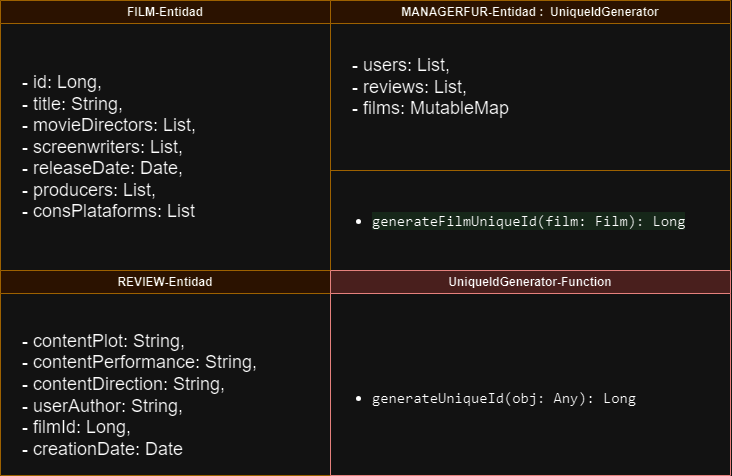
\includegraphics[width=\linewidth]{imagenes/Modelo_Dominio_Claqueta_TFG.drawio.png}
    \caption{Modelo de dominio.}
    \label{fig:diagrama}
\end{figure}



Como base y resumen del modelo de dominio, se tiene una entidad \begin{otherlanguage}
{english}\textit{\textbf{review }}\end{otherlanguage}haciendo referencia a la reseña, la entidad 
esencial, ya que se persigue asegurar la calidad de esta. Una reseña de calidad va a ser definida 
comúnmente como una reseña fiable que cumpla las reglas que se vieron en el estado del arte. Por lo tanto, 
estará formada por atributos generales como un identificador que la relacione con la 
película a la cual está criticando y otro para identificar al usuario que la ha escrito, la fecha de 
realización de esta crítica y también el contenido de la reseña se dividiría para que el usuario hable tanto de la 
trama general, la interpretación y la dirección. Asegurando las reglas vistas en el estado del arte.

Otra entidad importante es la \begin{otherlanguage}{english}\textit{\textbf{film }}\end{otherlanguage} 
siendo su propuesta mínima un conjunto de atributos que definen el contenido de dicha película como los 
directores, los guionistas, la fecha de estreno, las productoras y las plataformas en las que se puede 
consumir dicha película. Este conjunto de atributos es indispensable para la recomendación de dicho 
contenido, siendo cada uno puntos en común que buscar en otras películas para sus recomendaciones 
personalizadas. Evidentemente, también se necesita el título de la película y un identificador, ya que el 
resto de atributos puede coincidir y no identificar de manera única a la película.

Por último, existe una entidad que se encarga de gestionar tanto películas, como reseñas, como 
usuarios. Además, hace uso de una función que nos permitirá generar el identificador único para cada 
película y otros objetos que lo puedan necesitar.

\subsection{Lenguaje de programación}

Una de las principales herramientas para el desarrollo de software es el lenguaje de programación, un 
lenguaje que sea afín a las necesidades del proyecto. Siendo así necesario un lenguaje para modelar 
los objetos descritos en este capítulo, en el primer hito. Pero hay que tener en cuenta que se pretende 
que el desarrollo del modelado de los objetos pueda ser reutilizable, de fácil acceso e intentando 
ahorrar recursos. Por ello, se podría diseñar una API propia, como las que se 
mencionaron en el capítulo del estado del arte. Ya que es muy atractivo que los algoritmos y el modelo 
de datos pueda ser consumido por otros a través de una API

Por ahora se debe encontrar un lenguaje que sea flexible y que se adapte a las necesidades del proyecto. Con 
lo que se busca un lenguaje de propósito general, lo cual permitirá crear diversos proyectos. 
Siendo estos más sencillos de implementar en unos lenguajes que en otros. Se podría pensar en lenguajes 
como Java, Groovy, Scala o Kotlin. Siendo todos ejecutados en la máquina virtual de java (JVM), siendo 
Java, el veterano, es robusto y multiplataforma, pero su sintaxis puede ser un tanto prolija. Kotlin, 
por su parte, destaca por ser moderno, conciso y compatible con Java, además de ofrecer avanzadas 
características de seguridad. Aunque Groovy simplifica la sintaxis, su velocidad de ejecución más lenta 
podría ser un inconveniente. Scala, con un enfoque en la programación funcional, es expresivo, pero 
puede presentar una curva de aprendizaje más pronunciada. En conclusión, Kotlin emerge como la elección 
óptima en la JVM debido a su curva de aprendizaje suave, su amplia gama de bibliotecas y su excepcional 
interoperabilidad con Java, presentando una combinación equilibrada de simplicidad y funcionalidades 
avanzadas. 

\subsection{Testing}

Un proyecto con un enfoque ágil está sujeto a pruebas constantemente, algo que se está apegando en este 
proyecto a los PMVs resultantes de los milestones. De esta manera, se asegura la 
calidad del producto y se cerciora su funcionamiento. Consiguiendo así productos de 
calidad más robustos y minimizando errores.

Como se ha mencionado, Kotlin goza de acceso a un extenso conjunto de librerías y \textit{frameworks}. 
En este conjunto existen varios \textit{frameworks} que nos permiten testear el código.

Una herramienta esencial para fortalecer el proceso de desarrollo, las pruebas de flujo de trabajo con Docker 
\cite{GI_act}. Esta herramienta permite llevar a cabo pruebas exhaustivas de los flujos de trabajo de manera 
local antes de su implementación en el entorno remoto, destacándose por su integración efectiva con Docker. La 
característica distintiva de esta herramienta radica en dicha capacidad para generar simulaciones precisas, 
lanzando y evaluando flujos de trabajo en un entorno controlado basado en Docker. Asegurando la funcionalidad y 
consistencia de los flujos de trabajo antes de su inclusión en el entorno remoto, proporcionando la confianza 
necesaria en la calidad del código. Siendo una herramienta clave para garantizar una implementación sin 
contratiempos, mejorando la robustez y la calidad de los flujos de trabajo antes de su despliegue.

Para test unitarios del código existen varios \textit{frameworks}, por un lado,  
\textit{Spek}\footnote{\url{https://github.com/spekframework/spek}}. Una herramienta escrita para 
Kotlin diseñada para facilitar la escritura y ejecución de pruebas en proyectos escritos en este 
lenguaje. Permite definir pruebas en un estilo legible similar al lenguaje natural, lo que facilita 
su comprensión tanto para desarrolladores como para no desarrolladores. Por ello, algunos 
desarrolladores lo relacionan con \begin{otherlanguage}
{english}\textit{Behavior-Driven Development}\end{otherlanguage} (BDD), desarrollo guiado por 
comportamiento. Aunque sus creadores ya han mencionado 
\footnote{\url{https://spekframework.github.io/spek/docs/latest/}} que creen que hay una falsa 
distinción en torno al desarrollo guiado por comportamiento (BDD) y el desarrollo guiado por pruebas 
(TDD). Por lo que recomiendan que se piense en Spek como un simple \textit{framework} de 
especificación.

También se dispone de la herramienta por defecto que incorpora cualquier tipo de proyecto Kotlin, 
\textit{JUnit5}. Este es la última versión del \textit{framework} de pruebas unitarias para Java. Posee 
una arquitectura modular que se compone de tres módulos principales: JUnit Platform, JUnit Jupiter y 
JUnit Vintage, el primero es el núcleo de la herramienta, el segundo introduce las anotaciones y 
permite configurar los test, y la última permite la compatibilidad con versiones anteriores de este 
\textit{framework}. Este es el más usado actualmente por los desarrolladores 
\footnote{\url{https://www.jetbrains.com/es-es/lp/devecosystem-2022/testing/}} como nos indica 
\textbf{\textit{Jetbrains}}, compañía que ha diseñado Kotlin.

Ambos son buenas herramientas de pruebas. Además, permiten la integración con otras bibliotecas o 
\textit{framework} de pruebas. Pero ambas herramientas necesitan de otras bibliotecas imprescindibles 
en las pruebas, estas permiten simular objetos de una clase para trucar el resultado de ciertas 
funciones que se quieran testear. Estos objetos se denominan \textbf{\textit{Mock}}, en Kotlin 
se encuentra la librería nativa \textit{mockk}. Con uno de los \textit{frameworks} 
mencionados y esta librería se podrian realizar los test unitarios que se necesiten. Por lo que principalmente 
si no en su totalidad se usara Junit5 debido a la cantidad de información y ejemplos de uso, además de 
ser la herramienta usada por la mayoría de desarrolladores.

Para la parte de testeo de UI existe acceso a varias herramientas, pero se usará el 
\textit{framework} \textbf{\textit{Espresso}}\footnote{\url{https://developer.android.com/training/testing/espresso?hl=es-419}}, una herramienta creada por Google y la más recomendada \cite{UITest}.

Por último, si fuera necesaria una herramienta para testear las operaciones de una API, para  recuperar, 
insertar, modificar o eliminar información. Como se ha visto entre 
las herramientas más usadas para las pruebas\footnote{\url{https://www.jetbrains.com/es-es/lp/devecosystem-2022/testing/}} se encuentra \textit{\textbf{Postman}} una página para ayudar a los 
desarrolladores de API. Por ello es la herramienta que se usara en tal caso para realizar dichas 
pruebas, además es sencilla y cómoda de usar.

\section{M2: Lógica de negocio - Operaciones sobre los datos}

En este hito \footnote{\url{https://github.com/JoseJordanF/Claqueta/milestone/3}} se hablará de la 
lógica de negocio, también conocida como reglas de negocio, estas se refieren a las operaciones y procesos 
fundamentales que definen cómo funciona la aplicación. Determinando como se procesan los datos, se 
realizan cálculos, se toman decisiones y se llevan a cabo las operaciones clave para lograr los 
objetivos de la aplicación. Siempre dependientes de las necesidades y los propósitos de la aplicación. 
Estas vienen definidas por las \textbf{Historias de Usuario}, por lo que se va a recurrir a ellas para 
determinar las operaciones que se llevaran a cabo sobre los datos. Se promoverá la correcta 
implementación de la lógica de negocio, asegurando la coherencia y validez en las operaciones a través 
de los test unitarios. Siguiendo como siempre la esencia del desarrollo ágil, asegurando las
buenas prácticas para garantizar la calidad del proyecto, teniendo en cuenta que la lógica de negocio es 
el núcleo esencial que da vida a una aplicación y hace posible su funcionalidad y utilidad. 

Cabe destacar que lo primero que se hará es crear un proyecto Kotlin creado por gradle, un sistema de 
automatización de construcción de código de software por defecto, en este caso en IntelliJ IDEA. Esto 
es imprescindible, ya que para una mayor comodidad en la configuración y el uso de las distintas 
herramientas que nos ofrece Kotlin es necesario la creación de un proyecto.

Por otro lado, se necesita un flujo de trabajo que permita seguir unas buenas prácticas comprobando
la calidad del código escrito en dicho lenguaje. Cada cambio, cada nueva incorporación al código, asegurando
su calidad, velando por los principios del enfoque ágil, mencionados en el primer capítulo. Para ello se busca un 
linter o analizador estático de código, siendo este una herramienta que revisa el código en busca de posibles 
errores, malas prácticas o incumplimientos de estilo antes de que se ejecute. Este enfoque proactivo no solo 
ayuda a prevenir problemas antes de que afecten el rendimiento o la funcionalidad del software, sino que 
también se alinea perfectamente con los principios ágiles al fomentar la iteración continua y la mejora 
constante del código, promoviendo así un desarrollo más ágil y eficiente. 

Para la creación de este flujo de trabajo se necesita un linter para Kotlin que compruebe los ficheros con 
extensión de archivo Kotlin(.kt). Y hacer esto cada vez que se añada un nuevo archivo Kotlin al repositorio 
o se modifique alguno ya existente en algún pull request. Para esta tarea es mucho más rentable usar GitHub 
Actions, ya que debido a su amplia comunidad es sencillo encontrar un linter para el lenguaje que se prefiera. 
Por otra parte, la creación del flujo es prácticamente instantánea debido a la guía por parte de GitHub y el conocimiento previo que se tenía de estos al haber usado antes dicha herramienta. 
También es una tarea sencilla y poco pesada para que GitHub Actions la lleve a cabo, y no ocasiona gastos 
adicionales.
A continuación, cada una de las siguientes secciones representa un conjunto de issues que se han resuelto para obtener 
un PMV.

\subsection{Identificación y creación de las películas}

Una vez creado el proyecto con los modelos de dominio, se comienza a pensar en las 
distintas operaciones sobre los datos. Para empezar se debería preguntar qué contenido van a 
consumir los usuarios, claramente películas y en sí las reseñas de estas. Por lo tanto, primeramente 
hay que diferenciar de manera única cada película. Para ello es necesario el identificador de cada 
película, pero aún no se ha definido como se creara dicho identificador. Para generar este 
identificador se puede optar por múltiples opciones, se podría pensar en usar el título de la película 
o el nombre de alguno de los directores. Pero esto lleva a un problema debido a 
que existen películas que poseen el mismo título y son diferentes, al igual que los directores. 
Incluso se puede llegar a dar la casualidad de que existan dos películas con el mismo título y 
un director en común, siendo estas diferentes. Por lo tanto, no se podría usar el título y algún 
director, o al menos si solo se usan estos datos. Por lo tanto, esta deja de ser una posibilidad, aún 
hay muchas más opciones, se podría recurrir a la base de datos para generar un identificador 
único, ya que muchas bases de datos modernas poseen esta función incorporada. Pero no se quiere 
depender de la base de datos para generar estos identificadores, ya que en este punto del proyecto no 
es necesaria la base de datos. De manera que existen otras opciones como GUID una implementación de 
Windows para generar identificadores siguiendo un algoritmo específico, o alguna otra opción como los 
métodos que usan una marca en el tiempo y un identificador para cada nodo en el sistema. La comparación 
entre ambas opciones \cite{compSnowUUID} deja ver que las opciones estilo UUID son valores de 128 bits 
y no tienen un criterio determinado para generar dicho identificador, mientras que los métodos estilo 
snowflake son valores enteros de 64 bits y tienen una forma determinada de generar dicho identificador. 
Debido a la facilidad de seguir un algoritmo determinado y que no se necesita representar demasiados 
datos como para usar 128 bits, se ha decidido usar snowflake \cite{snowF} método creado por Twitter. 
Básicamente, se basa en crear un identificador único representado en decimal por número binario creado 
por bloques, el primero de 41 bits que define los milisegundos pasados desde una marca de tiempo 
determinada, el segundo bloque de 10 bits representa un identificador propio del objeto, en este caso 
se ha decidido fusionar el título de la película y el nombre del primer director para crear un número 
de 10 bits para este bloque. Por último, el bloque final de 12 bits que simplemente represente un 
número de secuencia por si se da la casualidad que se crean varios objetos en el mismo milisegundo y 
con el mismo título y primer director. Dándonos un identificador que cumple con las necesidades de 
sobra.

\subsection{Que es el consumo, quién lo consume y como lo lleva a cabo}

Tras resolver este problema para identificar el contenido, se puede pasar a definir como crear ese 
contenido por parte de la entidad que administra todo. Para ello, cada vez que se crea una película, 
además de introducir todos los datos requeridos, se crea su identificador y se añade a la lista de 
películas del proyecto. Ahora bien, para que este contenido pueda ser consumido por los usuarios, estos
deben estar creados en el sistema, por tanto, se define como se crea un usuario y se introduce 
en la lista de usuarios. Esto lleva a responder como se define el consumo y como se designa que un 
usuario ha consumido, en este caso una película. Lo que lleva a una interacción por parte del 
usuario para responder a esas preguntas, definiéndose ese consumo como la creación de reseñas por parte de este.
Siendo las películas en las que reseña o en las que interactúa con las reseñas de alguna manera, las películas que 
consume el usuario. Esto es algo que se definirá más adelante en la lógica de negocio. 

\subsection{Creación de reseñas}

Una vez creadas las películas y los usuarios, se necesita definir como se crean las reseñas a través de 
los datos necesarios, la relación con la película y el usuario que la ha escrito. Ya que se tiene todo 
lo necesario para la creación de esta reseña. Dando lugar a la reseña en sí misma y a la marca del 
consumo por parte del usuario, tema mencionado justo en la sección anterior. Además de comprobar que no 
exista una reseña de esa película ya escrita por este usuario, ya que cada usuario solo puede escribir 
una reseña por película.

\subsection{Recomendación de contenido al usuario}

Definido el consumo como la realización de reseñas por parte del usuario, se toma esto como marca 
de consumo. Siendo el consumo del usuario, todas las películas en las que ha 
reseñado estas servirán para la creación de sus recomendaciones. Las recomendaciones 
se harán a través de los datos comunes de estas películas, los directores, las productoras, los guionistas o las 
plataformas donde se pueden ver estas películas. Cualquiera de estos datos se utilizará para recomendar cualquier 
película que no se haya consumido y tenga algún dato en común con el consumo del usuario. De esta manera 
se obtendría una lista de películas recomendadas para el usuario sin repetidos, ya que es posible que varios datos 
coincidan en las mismas películas. Esta lista se refrescará cada vez que el usuario escriba una reseña 
en una nueva película.

Por cada una de estas operaciones se pueden dar varios casos de uso que se han estudiado a través de 
los test unitarios. Comprobando que cada caso de uso se lleva a cabo como se espera y el conjunto de 
ellos también. Para proseguir con las buenas prácticas y asegurar la calidad del proyecto y de su desarrollo, 
se deben seguir los principios vistos en la introducción sobre enfoque ágil, proporcionando una calidad mayor al 
proyecto y obteniendo un mayor control sobre su desarrollo. Es por esto que se debe crear un flujo de trabajo 
que permita la ejecución de los test unitarios cada vez que se realice un cambio en los ficheros Kotlin del 
proyecto. Por lo tanto, es necesario decidir que herramienta de integración continua se va a usar para ello. 
GitHub Actions puede usarse perfectamente para la creación del flujo, al igual que se usó para el flujo del 
linter, ya que solo se necesita ejecutar test unitarios simples que pueden ser ejecutados en una máquina virtual 
Ubuntu y en este caso para asegurar el correcto funcionamiento de estos, son ejecutados sobre distintas 
versiones de Java.

\section{M3: Servicios esenciales para la aplicación}

En este hito \footnote{\url{https://github.com/JoseJordanF/Claqueta/milestone/9}} se busca dotar a la aplicación de
dos funcionalidades esenciales para esta, siguiéndose el problema planteado por el desarrollador 
\footnote{\url{https://github.com/JoseJordanF/Claqueta/issues/125}}. De esta manera, primero se debe buscar una 
herramienta para el primer servicio, que según lo expuesto por el desarrollador, debe ser una herramienta que 
permita gestionar la configuración de la aplicación; pudiéndose obtener lo necesario para el arranque de la aplicación 
y su posterior funcionamiento. Esta herramienta debe ser capaz de cargar esta configuración desde distintas fuentes, 
velando por el arranque de la aplicación, ya que como menciona el desarrollador, estos ficheros pueden ser de 
distintos tipos, luego afiliarse a uno solo podría llevar a una carga errónea de este y que la 
aplicación no funcionase. Por lo que se ha recurrido a las fuentes más populares en aplicaciones Kotlin 
\cite{popularConfig} como JSON\cite{JsonWiki}, ficheros Java Properties\cite{JProWiki}, YAML\cite{YmlWiki}, 
HOCON\cite{HoconWiki} o ficheros INI\cite{IniWiki}. Esta sería una de las fuentes independientemente del tipo de 
archivo, otra indudable fuente y más habitual, son las variables de entorno, aunque en lenguajes de la JVM como 
Kotlin aparece otra fuente similar a las variables de entorno; en este caso se trata de las propiedades
del sistema, en sí de la JVM 
\footnote{\url{https://docs.oracle.com/javase/tutorial/essential/environment/sysprop.html}}. Con estas tres fuentes
se puede crear una jerarquía de lectura según las practicas más habituales en los lenguajes de la JVM 
\footnote{\url{https://docs.appdynamics.com/appd/4.5.x/en/application-monitoring/install-app-server-agents/java-agent/administer-the-java-agent}}, en este caso en Kotlin, así se seguirá la siguiente jerarquía, la primera fuente 
será las variables de entorno del sistema, si esta falla se recurrirá a las propiedades del sistema 
\cite{SecrectsJavaP} y por último se recurrirá al archivo de configuración.

Para Kotlin existen mucha variedad de bibliotecas para controlar la configuración de la aplicación, pero se busca 
una que permita el máximo número de fuentes vistas antes, e incluso que permita leer variables de entorno y archivos 
dotenv. Se busca principalmente en el repositorio oficial de Maven \footnote{\url{https://mvnrepository.com/}}, ya 
que brinda una gran cantidad de opciones, además de más información relacionada con la popularidad de la biblioteca 
o las vulnerabilidades que estas tienen. Las bibliotecas encontradas serían las siguientes, Apache Commons 
Configuration\footnote{\url{https://commons.apache.org/proper/commons-configuration/}}, Config de 
Lightbend\footnote{\url{https://github.com/lightbend/config}}, Config 
Magic\footnote{\url{https://github.com/brianm/config-magic}}, Config de 
NetworkNT\footnote{\url{https://mvnrepository.com/artifact/com.networknt/config/2.1.33}}, están listadas en orden de
popularidad, la mayoría tiene soporte para leer de distintas extensiones como JSON o YAML, pero pocas pueden leer de
más de una de estas extensiones; sin embargo, Config de Lightbend y  Config de NetworkNT poseen soporte nativo para 
JSON, ficheros Java Properties y JSON, YAML respectivamente. Pero desgraciadamente ninguna de ellas puede leer 
nativamente archivos dotenv, ni variables de entorno, ni propiedades del sistema. Por lo que se ha decidido usar una 
librería creada por el desarrollador\footnote{\url{https://github.com/JoseJordanF/LibraryConfigProject}}, la 
cual encapsula el funcionamiento de tres bibliotecas, una ya se conoce, ya que es una de las mejores opciones 
discutida arriba, Config de Lightbend que cubre JSON, Java Properties y HOCON, dotenv-
java\footnote{\url{https://github.com/cdimascio/dotenv-java}} que cubre las variables de entorno y los archivos 
dotenv y por último snakeyaml \footnote{\url{https://bitbucket.org/snakeyaml/snakeyaml/src/master/}} que cubre los 
archivos YAML. También de forma nativa lee propiedades del sistema y variables de entorno del sistema, de manera que 
dicha librería lee nativamente archivos JSON, Java Properties, YAML, HOCON e incluso dotenv, además encapsula la 
lectura de fuentes indispensables y más habituales, variables de entorno y propiedades del sistema, por ende es la 
herramienta perfecta para la aplicación.

De modo que la implementación de esta funcionalidad constara de una clase \begin{otherlanguage} {english}``\textit{\textbf{configurator}}''\end{otherlanguage} que permita cargar la configuración siguiendo la 
jerarquía comentada, y en cualquier momento permitir obtener dichos datos a través de dicha clase. Se necesita que
solo exista una instancia de esta clase, ya que simplemente se cargara la configuración al inicio de la aplicación, 
sin necesidad de más instancias, aportando control estricto sobre la única instancia, ya que la configuración,
trata con secretos delicados. A este patrón de diseño se le conoce como patrón singleton \cite{PattSingl}, en Kotlin 
existen algunas formas de conseguir esto \cite{SinglKotlin}, en este caso esto se logra marcando el constructor como 
privado, lo que evita la creación de instancias fuera de la propia clase. Además, se utiliza un objeto companion 
para almacenar esta única instancia y proporcionar un punto de acceso global a través de la clase. De esta manera, 
se asegura que cualquier parte del código pueda acceder a la misma instancia de \begin{otherlanguage} {english}``\textit{\textbf{configurator}}''\end{otherlanguage}, garantizando la coherencia de la configuración en 
toda la aplicación.

Para la segunda funcionalidad esencial, tal como menciona el desarrollador 
\footnote{\url{https://github.com/JoseJordanF/Claqueta/issues/126}}, se necesita una herramienta que permita 
registrar las distintas acciones de la aplicación para controlar el correcto funcionamiento de esta, y sobre todo 
los errores que se puedan dar durante su ejecución. También debe permitir el registro de la actividad de las 
acciones del usuario; dando estos registros por pantalla o en un archivo de registros, o incluso en ambos, con un 
formato descriptivo para una lectura clara del registro. En este caso, Kotlin o los lenguajes de la JVM poseen 
varias opciones populares, destacando del repositorio de Maven el módulo 
SLF4J\footnote{\url{https://www.slf4j.org/}}. Este módulo sirve de fachada o abstracción para distintos marcos de 
registro muy populares en estos lenguajes, como LogBack\footnote{\url{https://logback.qos.ch/documentation.html}}, 
Log4j 2\footnote{\url{https://logging.apache.org/log4j/2.12.x/}} o Apache Commons 
Logging\footnote{\url{https://commons.apache.org/proper/commons-logging/}}, siendo estos los más usados y populares 
dentro de la comunidad, tal como nos indica Maven\footnote{\url{https://mvnrepository.com/open-source/logging-frameworks}}. 
De esas tres bibliotecas, LogBack y Log4j 2 cumplen con los requisitos del desarrollador, ya que Apache Commons 
Logging carece de configuración que permita dar un formato específico a los logs o indicar la salida de estos, 
además es una fachada comúnmente usada para redirigir los mensajes de registro a SLF4J. Por lo tanto, cualquier 
biblioteca entre las dos mencionadas con anterioridad cumpliría con los requisitos, aun así la elección se va a 
decantar por LogBack, ya que es un poco más popular y usada que Log4j 2.

La implementación de esta funcionalidad será como la anterior, ya que también será una clase singleton 
\cite{DPatterns} llamada \begin{otherlanguage} {english}``\textit{\textbf{SimpleLogger}}''\end{otherlanguage}, en 
este caso, ya que pueden crearse múltiples implementaciones del logger sin perturbar el código. Siendo una clase 
singleton para tener control sobre la única instancia existente y que sea más eficiente, ya que será más fácil de 
mantener una sola instancia. Esta se encargará de inicializar el objeto responsable de los registros, indicando la 
configuración de la biblioteca, teniendo en cuenta donde se guardaran los logs, como lo harán y en que formato lo 
harán, esto se consigue gracias a una interfaz que permite definir los componentes necesarios en la configuración de 
la biblioteca, los cuales son el \begin{otherlanguage} {english}``\textit{\textbf{appender}}''\end{otherlanguage} y 
el \begin{otherlanguage} {english}``\textit{\textbf{encoder}}''\end{otherlanguage}, el primero es el encargado de 
donde y como guardar los logs, mientras que el segundo indica el formato en el que lo hacen. De esta manera se podrán 
hacer distintas implementaciones de estos métodos para disponer de diferentes tipos de logs.

Por otro lado, también se hace uso de una clase LoggerManager la cual se usa para inyectar la implementación de 
logger que se requiera sin perturbar la implementación en el resto del código. Por último se dará como válida esta
implementación si pasa los test unitarios correspondientes, estos permiten comprobar si sé crean los registros en 
distintas operaciones de la aplicación, de manera que se comprueba su creación y si su información es la que se 
espera. Así se demuestra que las clases que usan el logger lo están usando como deberían y se demuestra que la 
implementación del logger funciona. 

\section{M4: Refactorización para la mejora de prácticas en el manejo de estructuras de datos y errores}

En este hito se pretende realizar una refactorización basada en algunas historias del 
desarrollador,\footnote{\url{https://github.com/JoseJordanF/Claqueta/issues/132}}
estas aseguran un funcionamiento más óptimo de la aplicación mediante el uso de las mejores prácticas sobre las 
estructuras de datos, disminuyendo el número de operaciones, o haciendo que estas sean más eficientes. También por 
parte del desarrollador \footnote{\url{https://github.com/JoseJordanF/Claqueta/issues/129}} se pretende establecer una 
jerarquía de clase para los posibles errores que puedan ocurrir en la aplicación. De esta manera se obtendrá una 
refactorización del código actual en el que se siguen las mejores prácticas en el manejo de estructuras de datos y el 
manejo de errores, siendo este el PMV obtenido tras la validación de este hito

Para mejorar la eficiencia de la aplicación se ha recurrido al uso o al cambio de estructuras de datos, como por 
ejemplo las reseñas, anteriormente estaban localizadas en una lista de objetos \begin{otherlanguage} {english}``\textit{\textbf{Review}}''\end{otherlanguage}, 
pero esto lo hacía tremendamente ineficiente, ya que si se quisieran buscar las reseñas de un usuario o las reseñas 
de una película tendrían que localizarse recorriendo la lista. Pero haciendo uso de un diccionario\cite{OaksJava} que 
relaciona un identificador con un grupo de reseñas es eternamente más eficiente. Para ello se han realizado varios 
cambios, la forma de añadir un usuario comprobando que no existía ya uno con dicho nombre era bastante ineficiente, ya 
que requería recorrer la lista, por lo que se ha decidido usar un conjunto para guardar los usuarios. Así se 
han sobrecargado los métodos de conjunto\cite{BlochEffective} para considerar dos usuarios iguales si tienen el mismo 
nombre de usuario, de manera que agregar nuevos usuarios es más sencillo y más eficiente a la hora de comprobar si ya 
existe alguno con el mismo nombre de usuario.

Una vez hecho el cambio de los usuarios, al crear una reseña ahora se añaden dos entradas a la estructura de datos 
que las contiene, una representa las reseñas realizadas por el usuario y otra las reseñas referentes a una misma 
película. Así se tendría una eficiencia constante al realizar operaciones de búsqueda sobre dicha 
estructura\cite{LaforeData}; también se hace más eficiente la forma de comprobar si un usuario ya ha escrito una 
reseña sobre una película, ya que el conjunto de reseñas afiliado a esa clave del mapa que representa a una película o 
a un usuario, es un conjunto, de modo que también se sobrecargan los métodos del conjunto para designar una reseña 
igual a otra siempre que los identificadores que guarda dicha reseña sean iguales a los de otra. Así se impide la 
adición de reseñas repetidas porque en un conjunto de reseñas referentes a una película o aún usuario no puede haber 
más de una reseña con la misma ID de usuario o la misma ID de película, respectivamente. Estos cambios han supuesto 
que el resto de operaciones puedan modificarse para ser más eficientes.

Por otra parte, se ha introducido una jerarquía de clase para designar los distintos errores que pueden ocurrir
durante la ejecución de la aplicación, siendo perfectamente identificados los datos que los provocaron, a su vez 
también sé muestra el origen, y se usa un mensaje explícito para la comprensión del error. Su implementación se 
basa en la creación de clases que heredan de otras clases que manejan excepciones como lo es \begin{otherlanguage} {english}``\textit{\textbf{RuntimeException}}''\end{otherlanguage}, 
dependiendo del tipo de error se decidirá en cada momento de qué clase heredar.

Por último, se ha decidido crear una interfaz de la clase base \footnote{\url{https://github.com/JoseJordanF/Claqueta/issues/151}}
para facilitar la escalabilidad de la propia clase y la sencilla implementación de subtipos de ella, abogando por el 
principio de sustitución de Liskov visto en los principios SOLID.

Este hito se dará por válido si pasa todos los test unitarios dispuestos hasta ahora.


\section{M5: Acceso a los recursos de la API}

Antes de seguir con este hito, un pequeño inciso para aclarar que se tomó la decisión de no llevar a cabo la 
persistencia de datos y se dejara para una segunda refactorización, ya que por el momento la persistencia no es 
necesaria para responder a la historia del aficionado, por ende no forma parte de un PMV.

Ahora si en este hito se pretende llevar a cabo el diseño de la API estableciendo el  acceso a todos 
los recursos de la aplicación, ya sea para recuperar o crear objetos o acceder a la 
lógica de negocio. Por eso, en este hito se pretende buscar un framework que permita establecer rutas para acceder a los 
distintos recursos de la aplicación. Agregando valor para el desarrollador e indirectamente al cliente, pudiendo acceder 
a los recursos desde la aplicación cliente de forma sencilla y segura, dándose un PMV.

El desarrollador \footnote{\url{https://github.com/JoseJordanF/Claqueta/issues/137}} busca un framework con una
curva de aprendizaje llana, que sea modular\cite{modularSoft} para velar que su implementación sea ligera, 
también debe permitir que el formato de las respuestas pueda ser adaptado según las necesidades de la aplicación.
En este campo se pueden encontrar varias herramientas conocidas en el ámbito Java y Kotlin, como Spring 
Boot y Ktor respectivamente; siendo Ktor la herramienta por la que puede ser sustituida Spring Boot en un futuro 
\cite{ktorVSsboot}. En este caso ambas herramientas son modulares, pero el uso de Spring Boot es más complejo que el 
de Ktor, luego su curva sería más empinada, además el uso de Spring Boot no tiene sentido fuera de una aplicación 
basada en Spring\cite{springFrameW}. Por otro lado, Ktor también está guiada para aplicaciones ligeras y escalables, 
por lo que se va a usar Ktor como herramienta para el establecer el acceso a los distintos recursos de la API y el 
posible despliegue futuro.

Para la implementación se ha creado un módulo encargado de inicializar la configuración de las rutas para 
ofrecer respuestas a las distintas peticiones, además sé configura el servidor para probar las rutas de 
manera sencilla. 

Por otra parte, se añade la implementación de una clase donde se define la API con métodos centrados en los recursos,
como las películas, el detalle de una película, las reseñas de una película o las recomendaciones de un usuario. De
esta manera se han diseñado las rutas siguiendo las mejores prácticas \cite{RestPract} como respetar el nombre de los 
puntos finales, para que no contengan verbos ni acciones, ya que para diferenciar entre operaciones sobre dichos 
puntos finales se encuentran los verbos HTTP\footnote{\url{https://en.wikipedia.org/w/index.php?title=HTTP&ref=hackernoon.com##Request_methods}}. 
Y también se cuida que cada recurso sí es necesario este bajo otro recurso, dando sentido y describiendo el punto 
final.  Recurriendo a los recursos a través de los métodos de la clase mencionada, además, al principio del 
código de las rutas se ha incluido el complemento de Ktor para permitir que la salida de todas las peticiones sea en 
formato Json.

Para la validación de este hito será necesario que se compruebe con tests las peticiones a los distintos recursos, 
tanto el contenido como el mensaje de estado.

\section{M6: Aplicación cliente}

En este hito se quiere obtener una visión de la aplicación cliente, de forma que el PMV obtenido será una maqueta 
donde se pueda apreciar su funcionamiento, no un producto extensivo, el cual se dará en un hito posterior. Este PMV 
ofrecerá gran valor al desarrollador y al usuario, ya que podrá dar una vista a la interfaz que entrara en contacto 
con la API y con la que el usuario podrá satisfacer sus necesidades.

Por tanto, atendiendo al desarrollador \footnote{\url{https://github.com/JoseJordanF/Claqueta/issues/158}} se buscan 
herramientas que permitan el desarrollo de esta aplicación cliente, para ser escogidas deberán poseer una curva de 
aprendizaje llana, y ser bastante conocidas y usadas actualmente para tener acceso a los distintos conocimientos 
compartidos por la comunidad de desarrolladores. Siendo así más fácil la implementación para con los posibles errores 
que se puedan dar.

Como primera instancia se disponen dos herramientas omnipresentes en el desarrollo web, 
HTML\cite{WikiHtml}/CSS\cite{WikiCss}, ya que son dos pilares presentes en todas las herramientas usadas para llevar 
a cabo la construcción y el diseño de páginas web, ya que estas otras herramientas simplemente son abstracciones para 
trabajar a un nivel más alto, pero siempre mantienen dichos pilares bajo el capo. Siendo el fin conseguir un PMV se 
usará HTML/CSS puro, ya que su curva es llana al principio\cite{BookHtmlCss} y son herramientas ampliamente utilizadas
\footnote{\url{https://survey.stackoverflow.co/2023/##technology-most-popular-technologies}}. El diseño y la 
estructura de la página están cubiertos, pero aún se necesita una herramienta que permita hacer peticiones a la API 
para mostrar los datos en la página. Para realizar estas acciones se encuentran algunas opciones como 
JavaScript(JS)\cite{WhatIsJS}, TypeScript(TS)\cite{WhatIsTS} o Dart\cite{WhatIsDart}, si se comparan las curvas de 
aprendizaje, la de JS es bastante baja al comienzo, a diferencia de TS que es un poco más pronunciada aún siendo un 
superconjunto de JS, pero es más complejo debido al tipado estático, por último la curva de Dart es relativamente 
baja como JS. Ahora sí, si se pasa a ver el uso de cada uno 
\footnote{\url{https://survey.stackoverflow.co/2023/##technology-most-popular-technologies}},
se puede observar que distinguidamente JS es el más usado, seguido de TS y por último Dart, que no tiene mucho 
sentido usar si no lo haces junto a Flutter. Por lo que junto a HTML/CSS se usara JavaScript para la obtención de la 
primera vista de la aplicación cliente.

Para la implementación, se dispone de distintos archivos, el archivo.html donde se describe la estructura de la 
página, el archivo.css donde se describe el diseño de la página, y los archivos.js donde se describen las distintas 
acciones interactivas que ocurren durante el uso de la página. Una decisión destacada de esta sección, dada por un 
problema del usuario \footnote{\url{https://github.com/JoseJordanF/Claqueta/issues/159}}, viene a decir que el 
usuario tiene una imagen distintiva para ponerle cara a las películas en una web, cara que no se ha tenido en cuenta 
hasta ahora porque no ha sido necesaria; pero ahora es imprescindible que el usuario ponga cara a las distintas 
películas listadas, por lo que se ha decidido darles la vista común que espera el usuario, la portada de la 
película. Para ello no ha sido necesario perturbar ningún código anterior, simplemente se usan los datos de los que 
ya se disponen, una vez se solicitan desde la aplicación cliente se recurre a una API gratuita
\footnote{\url{https://developer.themoviedb.org/docs/getting-started}} que guarda las imágenes de estas películas, 
gracias a que se dispone del título y el año de estreno de cada película se puede obtener la imagen correspondiente.

\section{M7: Despliegue de prueba}

Para este pequeño hito se quiere realizar un despliegue de prueba de ambas aplicaciones, según el desarrollador 
\footnote{\url{https://github.com/JoseJordanF/Claqueta/issues/161}} se necesita encontrar una plataforma gratuita que 
permita subir la API en un contenedor\cite{BenefDocker}. Aparentemente, podría haber muchas opciones, pero la mayoría 
obligan a inscribirse a un plan de pago. Por lo que se ha encontrado la plataforma 
Railway\footnote{\url{https://docs.railway.app/overview/about-railway}}, la cual ofrece un mes gratuito y tiene soporte 
para desplegar contenedores o imágenes directamente de Docker. Por lo que ha sido escogida para el despliegue del back-
end, en cambio, no se ha conseguido desplegar mediante esta plataforma el front-end. Por lo que se ha recurrido a otra 
opción gratuita, 000Webhost\footnote{\url{https://www.000webhost.com/forum/about}} el cual está impulsado por 
Hostinguer\cite{WhatIsHostinger}; este ofrece un año gratis de hosting, y teniendo en cuenta que es un despliegue de 
prueba, entra dentro de nuestro PMV. Una vez descubiertas ambas plataformas, se desplegó primero la API obteniéndose un 
dominio generado por Railway\footnote{\url{https://api-node-production-493e.up.railway.app}}, por tanto, se cambió el 
código referente a las peticiones por parte de la aplicación cliente respecto a este nuevo dominio y también se desplegó 
\footnote{\url{https://claquetaweb.000webhostapp.com/}}. Actualmente ambas están desplegadas.

\section{Estimación de costes}

En esta sección se quiere realizar un cálculo estimado de los costes del proyecto, para ello se tienen que tener en 
cuenta distintos factores. Primero se debe tener en cuenta que ninguna herramienta usada ha requerido ningún gasto, ya 
que todas han sido de uso gratuito, siendo software libre o de código abierto. Por lo que el cálculo se centrara en la 
amortización del equipo usado para el desarrollo del proyecto, y el salario relativo del estudiante que realiza el 
proyecto. Primero se realizará el cálculo de amortización lineal del equipo\cite{CalcAmortizacion}:

\subsection{Amortización del equipo}

Respecto a los siguientes datos, se ha usado un PC que se compró hace un año por 1500€ y que según la agencia tributaria 
de España\cite{TablaAmortizacion} tiene una vida útil de 5 años y un coeficiente lineal máximo del 40\%. Se procede a 
calcular la amortización del primer año, ya que esta sería un valor residual para la de este año:
\begin{equation}
    1500\cdot0.4 = 600
    \label{Amortizacion primer año}
    \eqindex{Amortizacion primer año}
\end{equation}
De manera que la amortización del primer año serían 600€, este sería el valor residual de la amortización de este año dando lugar a que el valor del equipo para este año tras la depreciación sea:
\begin{equation}
    1500-600 = 900
    \label{Valor tras la depreciación}
    \eqindex{Valor tras la depreciación}
\end{equation}
Y sobre este valor se aplica el coeficiente lineal máximo:
\begin{equation}
    900\cdot0.4 = 360
    \label{Amortizacion del año del TFG}
    \eqindex{Amortizacion del año del TFG}
\end{equation}
Siendo la amortización de este año de 360€.

\subsection{Salario del estudiante}

Siendo realistas, se debe tener en cuenta que se está hablando de un estudiante sin experiencia, por lo cual se tomara
una media del salario de alguien con las mismas responsabilidades pero sin experiencia alguna. Según se puede 
comprobar\cite{WebSalary} el salario promedio en España para un desarrollador web sin experiencia seria de 30.324€ 
brutos al año, si se tiene en cuenta que se trabaja a jornada completa, luego 40 horas semanales, lo que daría 
redondeando 15€ por hora. Ahora se contempla que esto es una asignatura que ocupa un peso de 12 créditos y cada crédito 
es equivalente a 25 horas de trabajo 
\footnote{\url{https://www.educacionfpydeportes.gob.es/italia/dam/jcr:b53864d2-65a3-4526-abf4-61ef02f5be34/el-sistema-universitario-espa-ol2.pdf}} 
por lo tanto:
\begin{equation}
    12\cdot25 = 300
    \label{Calculo de horas teoricas}
    \eqindex{Calculo de horas teoricas}
\end{equation}
\begin{equation}
    300\cdot15 = 4.500
    \label{Sueldo basado en las horas estimadas}
    \eqindex{Sueldo basado en las horas estimadas}
\end{equation}
Lo que se resumiría en un salario de 4500€.

\subsection{Coste total}

Por lo que sí unimos los costes de amortización de este año y el salario del estudiante quedaría un coste de 4860€.
\begin{table}[h!]
\centering
\begin{tabular}{| m{15em} | m{10em} |}
 \hline
 \textbf{Concepto} & \textbf{Coste(€)} \\ 
 \hline
 Amortización del PC (primer año) &  600 \\ 
 \hline
 Amortización del PC (segundo año) &  360 \\ 
 \hline
 Salario (300 horas a 15€/hora)  & 4500 \\ 
 \hline
 \textbf{Total} & \textbf{4860} \\
 \hline
\end{tabular}
\caption{Estimación de Costes para el TFG}
\label{table:1}
\end{table}

	% Presupuesto

	% Conclusiones
	\chapter{Conclusiones y futuro del proyecto}

En este capítulo se verá si realmente se han cumplido los objetivos expuestos al comienzo del 
proyecto, en el caso de que lo hayan hecho, ver si la solución realmente ha sido óptima y los que aún no se hayan 
cumplido, como lo podrían hacer resumidamente. Y tratar alguna de las decisiones futuras del proyecto que estaría bien 
vislumbrar.

Al comienzo del proyecto se veía la necesidad del usuario por exponer su opinión referente al contenido consumido, en 
este aspecto se ha creado un sistema para la creación de reseñas fundadas, que de manera sencilla construye una reseña 
consistente describiendo aspectos fundamentales de cualquier película. También se mostraba el problema de indecisión 
entre la gente respecto a decidir que contenido cinematográfico iba a ver, debido a la cantidad de contenido existente, 
sin ninguna opción que conectara películas ya vistas con otras que les podían interesar. Por eso aparece en uno de los 
objetivos crear un algoritmo que sea capaz de recomendar a los usuarios contenidos según su consumo. Este es uno de los 
objetivos que se cree cumplido tras llegar al final del camino, ya que a través de las reseñas las recomendaciones le 
llueven al usuario, siempre conectadas de alguna forma con las películas ya consumidas y reseñadas. Otro de los 
objetivos que se cree cumplido es el de la creación de una aplicación para que el algoritmo de recomendaciones pueda ser 
consumido por los usuarios, además al crear una API indirectamente se puede apreciar una pequeña aportación para 
aquellos usuarios que quieran hacer uso del algoritmo en sus propias versiones de este proyecto, por lo que también 
sería consumido por desarrolladores.

Por otro lado, uno de los objetivos también era la creación de un algoritmo de fiabilidad de las reseñas. 
Lamentablemente con la solución actual no se ha podido lograr este objetivo, aunque un futuro próximo al proyecto podría 
conseguirlo. Ya que en la solución actual se ha podido satisfacer la historia del aficionado, la historia del cinéfilo 
tendría la clave para cumplir con el objetivo de lograr unas reseñas fiables, a través de distintos hitos, se obtendrían 
diversos PMV que terminaran cumpliendo con dicho objetivo y satisfaciendo las necesidades del cinéfilo. Es un objetivo 
que puede plantear varios problemas, pero que puede obtenerse a través de una solución no muy complicada, como sería el 
posible uso de un sistema de reputación como el existente en Stack Overflow. Permitiendo valorar al usuario cada reseña 
por el peso de la reputación del usuario que la haya escrito. Pero para obtener dicha solución, en este caso tendría que 
haberse solucionado el tema de la persistencia, ya que en la solución actual no ha sido necesaria, pero en esta 
situación para la integridad de los datos de reputación sería imprescindible.

Ya se discutiría que sistema de persistencia se usaría, relacional o no relacional, tratándose de un PMV en primera 
estancia y sin entrar en detalle se podría optar por una opción no relacional, ya que sería más flexible para el esquema 
pudiendo guardar las estructuras que se quiera mientras este más o menos bien organizado y la conversión para la 
respuesta de la API también podrían ser instantáneas siendo más sencilla su implementación. Además, ofrecen un gran 
desempeño para cargas de trabajo como realizar lecturas o escrituras rápidas y de un gran volumen de datos, gracias a 
poseer menos sobrecarga en la gestión de relaciones.

Aunque un sistema relacionar tampoco sería difícil de implantar aportando gran consistencia a los datos, permitiendo un 
mayor control sobre los datos y asegurando su consistencia. Pudiendo incluso sustituir el algoritmo de las 
recomendaciones por un conjunto de consultas complejas.

En un futuro se podría ver la elección de cualquiera de los dos sistemas, ya que ambos podrían ser implantados, la 
elección radicara en las necesidades del proyecto en ese momento, respecto a la escalabilidad de este, vertical u 
horizontal siendo un sistema no relacional o uno relacional la elección respectivamente.


	% Trabajos futuros


	
	\newpage
	\bibliography{bibliografia}
	\bibliographystyle{unsrt}
	
\end{document}

